%===============================================================================
% LaTeX sjabloon voor de bachelorproef toegepaste informatica aan HOGENT
% Meer info op https://github.com/HoGentTIN/bachproef-latex-sjabloon
%===============================================================================

\documentclass{bachproef-tin}

\usepackage{hogent-thesis-titlepage} % Titelpagina conform aan HOGENT huisstijl

%%---------- Documenteigenschappen ---------------------------------------------

% De titel van het rapport/bachelorproef
\title{Analyse van nummerplaatdetectie aan de parking van UGent Campus Sterre en Campus Coupure.}

% Je eigen naam
\author{Angelo Carly}

% De naam van je promotor (lector van de opleiding)
\promotor{Lotte Van Steenberghe}

% De naam van je co-promotor. Als je promotor ook je opdrachtgever is en je
% dus ook inhoudelijk begeleidt (en enkel dan!), mag je dit leeg laten.
\copromotor{Wannes Van Dorpe}

% Indien je bachelorproef in opdracht van/in samenwerking met een bedrijf of
% externe organisatie geschreven is, geef je hier de naam. Zoniet laat je dit
% zoals het is.
\instelling{VaDo Solutions}

% Academiejaar
\academiejaar{2019-2020}

% Examenperiode
%  - 1e semester = 1e examenperiode => 1
%  - 2e semester = 2e examenperiode => 2
%  - tweede zit  = 3e examenperiode => 3
\examenperiode{1}

%===============================================================================
% Inhoud document
%===============================================================================

\begin{document}

%---------- Taalselectie -------------------------------------------------------
% Als je je bachelorproef in het Engels schrijft, haal dan onderstaande regel
% uit commentaar. Let op: de tekst op de voorkaft blijft in het Nederlands, en
% dat is ook de bedoeling!

%\selectlanguage{english}

%---------- Titelblad ----------------------------------------------------------
\inserttitlepage

%---------- Samenvatting, voorwoord, woordenlijst --------------------------------------------
\usechapterimagefalse
%%=============================================================================
%% Voorwoord
%%=============================================================================

\chapter*{\IfLanguageName{dutch}{Woord vooraf}{Preface}}
\label{ch:voorwoord}

%% Het voorwoord is het enige deel van de bachelorproef waar je vanuit je
%% eigen standpunt (``ik-vorm'') mag schrijven. Je kan hier bv. motiveren
%% waarom jij het onderwerp wil bespreken.
%% Vergeet ook niet te bedanken wie je geholpen/gesteund/... heeft

Deze bachelorproef "Analyse van nummerplaatdetectie aan de parkingen op UGent Campus Sterre en Campus Coupure"\ werd geschreven met als doel het voltooien van mijn opleiding Toegaste Informatica aan de Hogeschool Gent. Dit onderwerp was tot stand gekomen nadat ik kennis vernam dat Vado-Solutions een dergelijk systeem aan het overwegen was in samenspraak met UGent. Dit sprak mij direct aan als een uitdagend onderwerp waar ik mijn kennis over GDPR en Artificial Intelligence kan bijschaven. Ik ben dan ook zeer dankbaar dat Vado-Solutions mij deze kans geschonken heeft.

Graag zou ik ook even de tijd nemen om enkele mensen te bedanken zonder wiens hulp en begeleiding deze bachelorproef niet tot stand zou gekomen zijn.

Eerst en vooral wil ik mijn co-promotors, Gino Van Dorpe en Wannes Van Dorpe, bedanken voor de steun en feedback in het maken van deze bachelorproef, evenals deze mooie kans om dit onderwerp te mogen uitvoeren.

Ook wil ik mijn promotor, Lotte Van Steenberghe bedanken om mij met nuttige feedback en ondersteuning goed op weg te zetten doorheen dit verhaal.

Ten laatste zou ik ook mijn ouders en medestudenten willen bedanken. In het bijzonder Simon Anckaert, Pieter Vandend3riessche en Shauni Van De Velde, om mij the helpen met morele steun en wijze feedback doorheen deze periode.
%%=============================================================================
%% Samenvatting
%%=============================================================================

% De "abstract" of samenvatting is een kernachtige (~ 1 blz. voor een
% thesis) synthese van het document.
%
% Deze aspecten moeten zeker aan bod komen:
% - Context: waarom is dit werk belangrijk?
% - Nood: waarom moest dit onderzocht worden?
% - Taak: wat heb je precies gedaan?
% - Object: wat staat in dit document geschreven?
% - Resultaat: wat was het resultaat?
% - Conclusie: wat is/zijn de belangrijkste conclusie(s)?
% - Perspectief: blijven er nog vragen open die in de toekomst nog kunnen
%    onderzocht worden? Wat is een mogelijk vervolg voor jouw onderzoek?
%
% LET OP! Een samenvatting is GEEN voorwoord!

%%---------- Nederlandse samenvatting -----------------------------------------

\IfLanguageName{english}{%
\selectlanguage{dutch}
\chapter*{Samenvatting}
%tekst
\selectlanguage{english}
}{}

%%---------- Samenvatting -----------------------------------------------------
% De samenvatting in de hoofdtaal van het document

\chapter*{\IfLanguageName{dutch}{Samenvatting}{Abstract}}

Tesamen met Vado-Solutions werd besloten om een onderzoek uit te voeren naar de mogelijkheid van nummerplaatdetectie op UGent op de Campussen Sterre en Coupure. De reden hiervoor was dat het huidige systeem met fysieke tokens die ingeworpen moeten worden niet gebruiksvriendelijk is en zou kunnen genieten van een vernieuwing. De nieuwe implementatie zou gebruiksvriendelijk, milieuvriendelijk en goedkoop moeten zijn.

Vado-Solutions had de interesse om hiervoor nummerplaatdetectie met een Raspberry Pi met PiNoIR camera en het open-source framework van OpenALPR te gebruiken. Deze hardware is uiterst goedkoop en zou een degelijke oplossing kunnen vormen, maar zekerheid hierover is niet altijd gegarandeerd. Dit onderzoek gaat na in welke mate dit mogelijk is op deze campussen van de UGent.

Het eerste deel van het onderzoek was het nagaan of een dergelijk systeem wel degelijk als legaal kan aanschouwd worden onder de huidige wetgeving van de GDPR. Deze was met oog op de voorgestelde implementatie van Vado-solutions zeker haalbaar. Iedere vorm van verwerken van persoonsgegevens dient gerechtigd te zijn en mogen enkel voor duidelijk omschreven doeleinden gebruikt worden. Verder is het verplicht om deze gegevens te kunnen opleveren of aanpassen indien gewenst van de eigenaar van de gegevens of enige autoriteiten. Deze verplichtingen hebben een grote implementatie- en onderhoudskost, wat niet gewenst is in een goedkope oplossing. Gelukkig blijkt dat indien er geen persoonsgegevens bijgehouden worden, niet aan deze voorwaarden voldoen kunnen worden. Dit brengt kosten omlaag en maakt een dergelijke implementatie mogelijk.

In het tweede deel zijn de mogelijke valkuilen voor een nummerplaatdetectiesysteem onderzocht in een literatuurstudie. Hieruit bleek dat een degelijke cameraconfiguratie van uiterst belang is. Een te lage resolutie, overbelichting of slechte invalshoek kunnen een drastische invloed hebben op de bekomen resultaten, en dienen met zorg ingesteld te worden.

Ten laatste werd er onderzocht of een fysieke implementatie wel degelijk haalbaar was op de locaties van UGent. Om dit te onderzoeken werden uitrijdende voertuigen op de vier uitgangen gefotografeerd met een Raspberry Pi met een PiNoir camera. Deze werden vervolgens verwerkt met OpenALPR, waarna de resultaten geanalyseerd werden. Uit de resultaten bleek dat gemiddeld 94.7\% van de voertuigen correct geïdentificeerd konden worden in rustige omstandigheden in daglicht. Deze resultaten zijn een geslaagd resultaat voor een steekproef en stellen de weg naar verder onderzoek open.

Uit dit onderzoek is gebleken dat nummerplaatdetectie mbv. een Raspberry Pi met PiNoIR-cam en OpenALPR wel degelijk mogelijk is om toegepast te worden op de uitgangen van UGent Campus Coupure en Campus Sterre. De voorgestelde implementatie van Vado-Solutions werd bevestigd om weinig tot geen invloed te ondervinden van de GDPR en een steekproef met veelbelovende resultaten was bekomen.

De resultaten van dit onderzoek stellen de weg open naar een breder onderzoek. Er is nog nood aan inzicht of deze resultaten ook 's nachts kunnen bekomen worden, zowel als de opties om een automatische cameratriggering te bekomen.


%---------- Inhoudstafel -------------------------------------------------------
\pagestyle{empty} % Geen hoofding
\tableofcontents  % Voeg de inhoudstafel toe
\cleardoublepage  % Zorg dat volgende hoofstuk op een oneven pagina begint
\pagestyle{fancy} % Zet hoofding opnieuw aan

%---------- Lijst figuren, afkortingen, ... ------------------------------------

% Indien gewenst kan je hier een lijst van figuren/tabellen opgeven. Geef in
% dat geval je figuren/tabellen altijd een korte beschrijving:
%
%  \caption[korte beschrijving]{uitgebreide beschrijving}
%
% De korte beschrijving wordt gebruikt voor deze lijst, de uitgebreide staat bij
% de figuur of tabel zelf.

\listoffigures
\listoftables

% Als je een lijst van afkortingen of termen wil toevoegen, dan hoort die
% hier thuis. Gebruik bijvoorbeeld de ``glossaries'' package.
% https://www.overleaf.com/learn/latex/Glossaries

%---------- Kern ---------------------------------------------------------------

% De eerste hoofdstukken van een bachelorproef zijn meestal een inleiding op
% het onderwerp, literatuurstudie en verantwoording methodologie.
% Aarzel niet om een meer beschrijvende titel aan deze hoofstukken te geven of
% om bijvoorbeeld de inleiding en/of stand van zaken over meerdere hoofdstukken
% te verspreiden!

%%=============================================================================
%% Inleiding
%%=============================================================================

\chapter{\IfLanguageName{dutch}{Inleiding}{Introduction}}
\label{ch:inleiding}

%De inleiding moet de lezer net genoeg informatie verschaffen om het onderwerp te begrijpen en in te zien waarom de onderzoeksvraag de moeite waard is om te onderzoeken. In de inleiding ga je literatuurverwijzingen beperken, zodat de tekst vlot leesbaar blijft. Je kan de inleiding verder onderverdelen in secties als dit de tekst verduidelijkt. Zaken die aan bod kunnen komen in de inleiding~\autocite{Pollefliet2011}:

%\begin{itemize}
  %\item context, achtergrond
  %\item afbakenen van het onderwerp
  %\item verantwoording van het onderwerp, methodologie
  %\item probleemstelling
  %\item onderzoeksdoelstelling
  %\item onderzoeksvraag
  %\item \ldots
%\end{itemize}

%Vandaag de dag heeft UGent enkele problemen met de toegangscontrole van hun parking. Het huidige systeem met tokens is een oude technologie en is aan vernieuwing toe.

\section{\IfLanguageName{dutch}{Probleemstelling}{Problem Statement}}
\label{sec:probleemstelling}

%Uit je probleemstelling moet duidelijk zijn dat je onderzoek een meerwaarde heeft voor een concrete doelgroep. De doelgroep moet goed gedefinieerd en afgelijnd zijn. Doelgroepen als ``bedrijven,'' ``KMO's,'' systeembeheerders, enz.~zijn nog te vaag. Als je een lijstje kan maken van de personen/organisaties die een meerwaarde zullen vinden in deze bachelorproef (dit is eigenlijk je steekproefkader), dan is dat een indicatie dat de doelgroep goed gedefinieerd is. Dit kan een enkel bedrijf zijn of zelfs één persoon (je co-promotor/opdrachtgever).

Vandaag de dag kampt UGent met problemen omtrent hun toegangssysteem aan de campus Coupure en campus Sterre. Het huidige systeem dat gebruikt maakt van tokens is niet efficiënt en zorgt voor veel extra werk. Enkele voorbeelden zijn:
\begin{itemize}
	\item De tokens moeten telkens afgehaald worden aan het onthaal om de campussen te kunnen verlaten.
	\item De tokenslikkers moeten regelmatig geleegd worden indien de tokenslikkers vol zijn.
	\item De tokens zijn relatief duur om bij te maken.
	\item De tokens worden snel kwijtgeraakt.
\end{itemize}
Door deze problemen overweegt UGent om op deze locaties over te stappen naar een beter systeem dat milieubewust is, beperkt in kostprijs is, en een goed gebruiksgemak heeft. 

Hierop biedt VaDo Solutions een innovatief systeem aan dat gebruik maakt van nummerplaatdetectie. Deze zou gebruik maken van een Raspberry PI in combinatie met een open-source library genaamd OpenALPR. Welke al reeds bevestigd zijn dat ze goede resultaten kunnen opleveren \autocite{figuerola2016automated}. Maar of deze resultaten ook haalbaar zijn op UGent zal nagegaan worden in dit onderzoek.

Verder heerst er enkele onduidelijkheid over hoe de GDPR inspeelt op een dergelijk systeem en welke maatregelingen er getroffen moeten worden.

\section{\IfLanguageName{dutch}{Onderzoeksvraag}{Research question}}
\label{sec:onderzoeksvraag}

%Wees zo concreet mogelijk bij het formuleren van je onderzoeksvraag. Een onderzoeksvraag is trouwens iets waar nog niemand op dit moment een antwoord heeft (voor zover je kan nagaan). Het opzoeken van bestaande informatie (bv. ``welke tools bestaan er voor deze toepassing?'') is dus geen onderzoeksvraag. Je kan de onderzoeksvraag verder specifiëren in deelvragen. Bv.~als je onderzoek gaat over performantiemetingen, dan 
Dit onderzoek zal nagaan in hoeverre het mogelijk is nummerplaatdetectie op te stellen op de Campus Coupure en Campus Sterre van UGent. Hiervoor wordt er bekeken in welke mate de GDPR invloed heeft op nummerplaatdetectie. Daarnaast zullen er maatregelingen opgesteld worden om een nauwkeurige detectie te verkrijgen, waarop er vervolgens een testopstelling gemaakt wordt om na te gaan of een dit wel degelijk mogelijk is op UGent.

Zo bekomen we volgende drie onderzoeksvragen:
\begin{itemize}
	\item Is nummerplaatdetectie een haalbare techniek omtrent privacy en GDPR?
	\item Welke maatregelingen moeten er genomen worden om succesvol nummerplaatdetectie te implementeren?
	\item Kan men nummerplaatdetectie succesvol uitvoeren met een Raspberry PI op de campus Coupure en Sterre van UGent?
\end{itemize}

\section{\IfLanguageName{dutch}{Onderzoeksdoelstelling}{Research objective}}
\label{sec:onderzoeksdoelstelling}

%Wat is het beoogde resultaat van je bachelorproef? Wat zijn de criteria voor succes? Beschrijf die zo concreet mogelijk. Gaat het bv. om een proof-of-concept, een prototype, een verslag met aanbevelingen, een vergelijkende studie, enz.

Dit onderzoek heeft als doel een correcte voorstelling te geven hoe nauwkeurig nummerplaatdetectie met een Raspberry Pi en OpenALPR uitgevoerd kan worden op UGent door hiervan een prototype te maken. Aan de hand van deze resultaten kan VaDo-Solutions beslissen of dit wel of niet de gewenste technologie is die ze willen gebruiken.

Vervolgens wordt er verwacht dat een duidelijk overzicht gegeven wordt van maatregelingen die getroffen kunnen worden om een dergelijk systeem te implementeren op vlak van hardware- en software-instellingen. Zo kan een installateur weten welke configuratie correcte resultaten kan leveren, zonder gebruik te moeten maken van trial-en-error.

Ten laatste is het de bedoeling om een bondige uitleg te hebben op welke vlakken de GDPR invloed heeft op dit soort camerasysteem. Hiermee kan een ontwikkelaar weten aan welke voorwaarden zijn opstelling moet voldoen zodat hij geen risico loopt op het overtreden van wetgevingen.

\section{\IfLanguageName{dutch}{Opzet van deze bachelorproef}{Structure of this bachelor thesis}}
\label{sec:opzet-bachelorproef}

% Het is gebruikelijk aan het einde van de inleiding een overzicht te
% geven van de opbouw van de rest van de tekst. Deze sectie bevat al een aanzet
% die je kan aanvullen/aanpassen in functie van je eigen tekst.

De rest van deze bachelorproef is als volgt opgebouwd:

In Hoofdstuk~\ref{ch:stand-van-zaken} wordt een overzicht gegeven van de stand van zaken binnen het onderzoeksdomein, op basis van een literatuurstudie.

In Hoofdstuk~\ref{ch:methodologie} wordt de methodologie toegelicht en worden de gebruikte onderzoekstechnieken besproken om een antwoord te kunnen formuleren op de onderzoeksvragen.

In Hoofdstuk~\ref{ch:wetgeving-nummerplaatdetectie} wordt er nagegaan waarop er gelet moet worden bij het implementeren van nummerplaatdetectie als toegangssysteem op vlak van privacywetgevingen.

In Hoofdstuk~\ref{ch:maatregelenanpr} wordt er nagegaan welke maatregelingen er genomen moeten worden om een zo performant mogelijke implementatie van nummerplaatdetectie te maken.

In Hoofdstuk~\ref{ch:praktischeUitvoering} wordt een onderzoek uitgevoerd aan de hand van de vooropgestelde maatregelingen aan de campus Sterre en Coupure van UGent. Hieruit zal blijken of nummerplaatdetectie met een Raspberry PI mogelijk is op deze locatie.

In Hoofdstuk~\ref{ch:conclusie}, tenslotte, wordt de conclusie gegeven en een antwoord geformuleerd op de onderzoeksvragen. Daarbij wordt ook een aanzet gegeven voor toekomstig onderzoek binnen dit domein.
\chapter{Stand van zaken}
\label{ch:stand-van-zaken}

% Tip: Begin elk hoofdstuk met een paragraaf inleiding die beschrijft hoe
% dit hoofdstuk past binnen het geheel van de bachelorproef. Geef in het
% bijzonder aan wat de link is met het vorige en volgende hoofdstuk.

% Pas na deze inleidende paragraaf komt de eerste sectiehoofding.

%Dit hoofdstuk bevat je literatuurstudie. De inhoud gaat verder op de inleiding, maar zal het onderwerp van de bachelorproef *diepgaand* uitspitten. De bedoeling is dat de lezer na lezing van dit hoofdstuk helemaal op de hoogte is van de huidige stand van zaken (state-of-the-art) in het onderzoeksdomein. Iemand die niet vertrouwd is met het onderwerp, weet er nu voldoende om de rest van het verhaal te kunnen volgen, zonder dat die er nog andere informatie moet over opzoeken \autocite{Pollefliet2011}.

%Je verwijst bij elke bewering die je doet, vakterm die je introduceert, enz. naar je bronnen. In \LaTeX{} kan dat met het commando \texttt{$\backslash${textcite\{\}}} of \texttt{$\backslash${autocite\{\}}}. Als argument van het commando geef je de ``sleutel'' van een ``record'' in een bibliografische databank in het Bib\TeX{}-formaat (een tekstbestand). Als je expliciet naar de auteur verwijst in de zin, gebruik je \texttt{$\backslash${}textcite\{\}}.
%Soms wil je de auteur niet expliciet vernoemen, dan gebruik je \texttt{$\backslash${}autocite\{\}}. In de volgende paragraaf een voorbeeld van elk.

%\textcite{Knuth1998} schreef een van de standaardwerken over sorteer- en zoekalgoritmen. Experten zijn het erover eens dat cloud computing een interessante opportuniteit vormen, zowel voor gebruikers als voor dienstverleners op vlak van informatietechnologie~\autocite{Creeger2009}.

% Huidige situatie UGent
Het huidige toegangssysteem aan UGent is een systeem op basis van tokens. Een bezoeker rijdt de parking op zonder enige checks. Vervolgens bezoekt hij de campus en vraagt een token om de campus te verlaten. Ten laatste rijdt hij zijn wagen naar de slagboom en geeft zijn token in de gepaste tokenslikker.

tokens: 
	veroudert simpelweg, moet buiten
	duur
	Personeelskosten: legen van tokenslikkers, tokens uitdelen

\textcite{aalsalem2015automated} beschrijft wat onveilig is aan rfid. (kopieren van kaarten)
studentenkaarten zijn rfid (?), maar niet iedereen heeft studentenkaart terwijl wel ieder voertuig nummerplaat heeft.
extra kosten! scanners, niet simpel te integreren (?), gelimiteerde administratieve trucjes.

anpr:
	heel modulair. mensen kunnen een dagpas krijgen, toegang kan simpel gerevoked worden. Weinig kosten. Nauwkeurigheid (?)
	Wat met snachts, regen, brommers, non-standaard nummerplaten. Is dit nog steeds de moeite dan?

gdpr:



OP TE ZOEKEN:
rfid veiligheid
rfid voordelen
rfid kost
anpr veiligheid?
anpr kost?
anpr voordelen?
anpr nadelen?
tokens nadelen?
tokens voordelen?
	
%%=============================================================================
%% Methodologie
%%=============================================================================

\chapter{\IfLanguageName{dutch}{Methodologie}{Methodology}}
\label{ch:methodologie}

%%  Hoe ben je te werk gegaan? Verdeel je onderzoek in grote fasen, en
%% licht in elke fase toe welke stappen je gevolgd hebt. Verantwoord waarom je
%% op deze manier te werk gegaan bent. Je moet kunnen aantonen dat je de best
%% mogelijke manier toegepast hebt om een antwoord te vinden op de
%% onderzoeksvraag.

In dit onderzoek wensen we inzicht te verkrijgen of een ANPR-systeem succesvol geïmplementeerd kan worden aan de parking van UGent op de campussen Sterre en Coupure. Ook wordt onderzocht welke maatregelen getroffen dienen te worden om zo'n systeem aan de GDPR te laten voldoen. Deze doelen werden opgesplitst in drie fasen en worden beschreven in de volgende hoofdstukken.

\section{Richtlijnen omtrent GDPR bij nummerplaatdetectie}
Sinds de GDPR vorig jaar is ingevoerd, moeten bedrijven veel meer rekening houden met hoe ze data verwerken. Deze richtlijnen zijn allemaal te vinden in de wettekst van de GDPR zelf, maar om deze te verduidelijken worden deze opgesomd.

Op basis van de richtlijnen die in dit hoofdstuk omschreven worden kan een ontwikkelaar inzicht krijgen in hoe een nummerplaatdetectiesysteem ingevoerd kan worden. Indien zo'n systeem deze richtlijnen niet volgt zal deze ook niet voldoen aan de GDPR. 

\section{Maatregelen voor nummerplaatdetectie met Raspberry Pi}
Een ANPR-systeem opzetten op een Raspberry Pi is niet vanzelfsprekend aangezien ANPR-systemen normaal met dure hardware worden geïnstalleerd. Om toch nauwkeurige resultaten te kunnen boeken, zal er in dit hoofdstuk beschreven worden wat de optimale waarden zijn in kwestie van camera-instellingen, plaatsing van de camera, netwerk.

A.d.h.v. deze maatregelen kan een ontwikkelaar een ANPR-systeem configureren met een zo hoog mogelijke nauwkeurigheid.

\section{Praktische uitvoering van nummerplaatdetectie op UGent}
Vervolgens kan er a.d.h.v. de vooropgestelde maatregelen getest worden of ANPR met een Raspberry Pi haalbaar is op UGent. Hiervoor zullen er op de campussen van de UGent foto's genomen worden met de Pi-Cam van voertuigen die de parkings willen verlaten. Hierbij zal er gekeken worden welke uitvoeringstijd de detectie nodig heeft. Achteraf wordt er per foto gecontroleerd of de gefotografeerde nummerplaat wel degelijk juist is gedetecteerd. Indien deze nauwkeurigheid hoog genoeg is, kan er besloten worden dat ANPR met een Raspberry PI een haalbare techniek is op UGent.

Voor het maken van de foto's zal gebruik gemaakt worden van de PiNoIR Camera, dit is een camera voor de Raspberry Pi die geen filtering heeft op infrarood licht, wat het optimaal maakt voor gebruik in donkere situaties \autocite{raspberrypisitemodelpinoir}.

% Voeg hier je eigen hoofdstukken toe die de ``corpus'' van je bachelorproef
% vormen. De structuur en titels hangen af van je eigen onderzoek. Je kan bv.
% elke fase in je onderzoek in een apart hoofdstuk bespreken.


\chapter{\IfLanguageName{dutch}{Richtlijnen omtrent GDPR bij nummerplaatdetectie}{Technical details about ANPR in the GDPR}}
\label{ch:richtlijnengdpr}

Algemene Verordening Gegevensbescherming (AVG)

gemaakt om gegevens omtrent natuurlijke personen te beschermen en is van toepassing 

\subsection{Persoonlijke data}
Wat is persoonlijke data?
alle informatie over een geidentificeerde of identificeerbare natuurlijke persoon.
identificeerbaar is wanneer een persoon direct of indirect kan worden geidentificeerd aan de hand van een indicator zoals naam adres, geboortedatum.

Dit houdt dus ook in nummerplaat, aangezien deze gelinkt is aan een persoon.


Wat willen we opslaan van persoonlijke data?
Must: nummerplaat
naam?
gsm?



Artikel 5 van GDPR, 'persoonsgegevens moeten worden verwerkt op een wijze die ten aanzien van de brotkkene rechtmatig, behoorlijk en transparant is ("rechtmatigheid, behoorlijkheid en transparantie").


\chapter{\IfLanguageName{dutch}{Maatregelen voor ANPR}{Implementation guide for ANPR}}
\label{ch:maatregelenanpr}

In deze sectie beoordelen we welke maatregelen genomen moeten worden bij het implementeren van een ANPR systeem met oog op de parking aan de UGent.

Nummerplaatdetectie is al sterk geevolueerd sinds vroeger, maar heeft nog steeds enkele drawbacks. Zo spelen factoren zoals weer, belichting en plaatsing van de camera's een invloed op de nauwkeurigheid van de uitlezingen.

%TODO deze alinea klopt niet, begint met een halve zin
zoals camerahoek, resolutie, weerstomstandigheden, belichting, afbeeldingcompressie, tijd voor een uitlezen. Door het volgen van deze maatregelen kan een werknemer nummerplaatdetectie installeren op een zo'n correct mogelijke manier.

\section{Camera Plaatsing}

\subsection{Locatie van de camera}
Uit een prototype van \textcite{arrieta2019prototype} bleek dat nummerplaten niet correct geïdentificeerd werden bij een inclinatiehoek vanaf 30 graden. Het is dus aanbevolen om de camerahoek te beperken tot een kleine hoek.

Verder is het aangeraden om de camera hoger te plaatsen dan de koplampen van de auto, dit om te voorkomen dat de camera verblind wordt door het sterke licht.

\subsection{Camera oriëntatie}
De gedetecteerde nummerplaten horen parallel te staan met de randen van de afbeelding. Dit omdat de datasets voor OpenANPR getraint zijn met afbeeldingen van horizontale nummerplaten, maar niet van gedraaide. Indien het niet mogelijk is om een rechte afbeelding te nemen kan de afbeelding ook later gedraaid worden.

\subsection{Pixeldichtheid}
Het aantal pixels van de foto waaruit een nummerplaat bestaat is van belang voor OpenALPR voor een duidelijke herkenning. Indien een foto van veraf is genomen zal deze laag zijn en van dichtbij zal deze dan weer hoog zijn. OpenALPR verwacht voor Europeaanse nummerplaten minstens een wijdte van 75 pixels en een grootte meer dan 250 pixels verhoogt niet opmerkelijk de accuraatheid. \autocite{openalprcameraplacement}

\section{Camera instellingen}
De belangrijkste factor van een performant ANPR-systeem is een correct ingestelde camera. Het nemen van foto's is de eerste stap in het proces en indien hierop nummerplaten niet duidelijk zijn kan OpenALPR onmogelijk iets detecteren. In dit onderdeel worden de belangrijkste instellingen verduidelijkt die bijdragen tot een correcte foto voor gebruik bij nummerplaatdetectie.

\subsection{Shuttersnelheid}
%\textcite{guo2017vehicle} stelt een trainingsmodel voor dat rekening houdt met blur.

Camera shutterspeed is de snelheid dat een camera foto's neemt. In een klaarlichte dag kan de shutterspeed zo'n 1/10000 seconden halen terwijl in het donker dit wel een volle seconde kan duren om genoeg licht te behalen. \autocite{openalprcameraplacement}

Bij een lange shutterspeed kan het dus zijn dat een voertuig een meter vooruit is gereden, terwijl bij een kleine shutterspeed dit bv. maar een centimeter is. Een korte shutterspeed is dus interessant voor het implementeren van nummerplaatdetectie aangezien de auto minder ver is gereden en dus minder motion blur op de foto staat.

\begin{figure}[h!]
	\centering
	\begin{subfigure}[b]{0.4\linewidth}
		\includegraphics[width=\linewidth]{img/shutter-slow.jpg}
		\caption{Shutter speed van 1/60}
	\end{subfigure}
	\begin{subfigure}[b]{0.4\linewidth}
		\includegraphics[width=\linewidth]{img/shutter-fast.jpg}
		\caption{Shutter speed van 1/250}
	\end{subfigure}
	\label{fig:ntlpc}
	\caption{Vergelijking van verschillende shutterinstellingen. \autocite{easy2019shutter}}
\end{figure}

Het nadeel van een kleine shutterspeed te nemen is dat er veel minder licht aanwezig is op de foto's, wat de detectie dan weer omlaag brengt. Zo krijg je 's nachts bijna volledig zwarte foto's. Dit kan geremedieerd worden door belichting bij te plaatsen.

\subsection{Belichting}
%TODO in dit onderdeel zou er nog een stuk ontbreken
's Nachts is de belichting van de nummerplaten een stoorzender, de camera kan onmogelijk een kleine shutterspeed aanhouden en een genoeg belichte afbeelding krijgen. Hiervoor moet er dus een eigen belichting bijgezet worden.

Zelfs al wordt er belichting bijgezet zal de nummerplaat spijtig genoeg niet leesbaar zijn, dit komt doordat de koplampen van een auto ervoor zorgen dat de camera niet eens een nummerplaat meer ziet. Een algemene oplossing voor deze problemen is het gebruik van een IR-camera. Een IR-camera detecteerd enkel IR-licht en heeft dus geen invloed van de koplampen van wagens. Verder is het voordeel hiervan dat IR-licht niet zichtbaar is voor het menselijk oog, en dus ongestoort snachts en overdag gebruikt kan worden.

\begin{figure}[h!]
	\centering
	\begin{subfigure}[b]{0.4\linewidth}
		\includegraphics[width=\linewidth]{img/night-time-lpc-bad.png}
		\caption{Slecht geconfigureerde camera.}
	\end{subfigure}
	\begin{subfigure}[b]{0.4\linewidth}
		\includegraphics[width=\linewidth]{img/night-time-lpc-good.png}
		\caption{Correct geconfigureerde camera.}
	\end{subfigure}
	\caption{Vergelijking tussen camerainstellingen in de nacht. \autocite{axis2019license}}
\end{figure}
Infrarood, infraroodlamp, dag, nacht

\subsection{Depth of field}
Om scherpe afbeeldingen te verkrijgen moet de depth of field (DOF) van een camera correct ingesteld staan. Deze bepaald in welke range een afbeelding scherp is. Hoe groter de DOF, hoe verder de objecten in focus zijn. Bij afstanden onder de 10m is de DOF aan de kleine kant en moet deze heel nauwkeurig ingesteld worden. \autocite{axis2019license}

\begin{figure}[h!]
	\centering
	\includegraphics[width=\linewidth]{img/depth-of-field.png}
	\caption{Verduidelijking van depth of field. \autocite{axis2019license}}
\end{figure}


\section{Configuratie}

\subsection{Pattern matching}
\textcite{arrieta2019prototype} en \textcite{buhus2016automatic} concluderen beiden dat openalpr standaard goede resultaten biedt, maar nog hogere resulaten bereikt kunnen worden indien er verduidelijkt wordt welk type nummerplaten er verwacht wordt. Dit houdt factoren in zoals de juiste dataset van het land gebruiken en de volgorde van de kentekenkarakters aanduiden.

Door pattern matching toe te passen kunnen resultaten nog nauwkeuriger zijn. Hierbij wordt een reguliere expressie op alle top N resultaten uitgevoerd en worden de non-matching resultaten verworpen.

Een voorbeeld hiervan is op nummerplaten in Tsjechië, verkregen van \textcite{openalpr2015pattern}
Er wordt nummerplaatdetectie uitgevoerd op afbeelding \ref{patternmatching} met volgende regexpatronen die voorkomen in Tsjechië:
\begin{itemize}
	\item cz \#@\#\#\#\#\#
	\item cz \#@@\#\#\#\#
\end{itemize}

\begin{lstlisting}
[mhill@mhill-linux tmp]$ alpr -c eu -p cz cz_4s50233.jpg -n 40
Config file location provided via default location
plate0: 40 results
- 4S5O233     confidence: 90.947      pattern_match: 0
- 4S5O23      confidence: 87.8683     pattern_match: 0
- 4S5O23      confidence: 85.1644     pattern_match: 0
- 4S5O23S     confidence: 84.5445     pattern_match: 0
- 4S5O23B     confidence: 83.7395     pattern_match: 0
- 4S5O2S3     confidence: 83.3698     pattern_match: 0
- 4S5O23G     confidence: 83.1375     pattern_match: 0
- 4S50233     confidence: 83.0457     pattern_match: 1
- 4S5O2B3     confidence: 82.5635     pattern_match: 0
- 4S5O2       confidence: 82.0857     pattern_match: 0
- 4S5O2G3     confidence: 81.5684     pattern_match: 0
- 4S5O2J3     confidence: 81.0409     pattern_match: 0
- 4S5O2S      confidence: 80.2911     pattern_match: 0
... more results that do not match ...
\end{lstlisting}

\begin{figure}[h!]
	\centering
	\includegraphics[width=\linewidth]{img/pattern-matching.jpg}
	\caption{Pattern matching van OpenALPR \autocite{openalpr2015pattern}}
	\label{patternmatching}
\end{figure}

Hieruit is te zien dat bij de top 7 resultaten het middelste karakter als een O zien i.p.v. een 0. Door te kijken of de pattern matching succesvol was, zien we dat het achtste resultaat correct is.

\subsection{Buitenlandse nummerplaten}
OpenALPR heeft verscheidene configuraties voor Europa, Amerika en andere continenten. Door één van deze te selecteren wordt een ander model gekozen dat specifiek voor deze regio getraint is. Bij een keuze van de Europese databank worden er dan ook geen tot weinig fouten verwacht indien een buitenlandse nummerplaat gedetecteerd is.

\subsection{Commerciële upgrades}
OpenALPR wilt ook wel winst maken en biedt dan ook een commerciële versie van OpenALPR aan, deze zou een hogere nauwkeurigheid bieden in enkele cases waar de Open Source versie slechte presteert. \autocite{openalpr2019benchmark}


\chapter{\IfLanguageName{dutch}{Praktische uitvoering van ANPR}{Implementation of ANPR at UGent}}
\label{ch:praktischeUitvoering}
In dit hoofdstuk wordt er onderzocht of nummerplaatdetectie degelijke resultaten kan behalen op de Campus Sterre en Campus Coupure van UGent. Hiervoor zullen handmatig foto's genomen worden van wagens die de parking verlaten a.d.h.v. een testopstelling van een Raspberry Pi met een Pi-NoIR camera. Vervolgens worden deze foto's verwerkt met OpenALPR en zullen deze resultaten vergeleken worden met de correcte resultaten. Op deze manier wordt de nauwkeurigheid van de nummerplaatdetectie per uitgang bepaalt en kan een conclusie getrokken worden of dit wel degelijk een haalbare technologie is.

\section{Opstelling}
In dit onderdeel wordt de opstelling en configuratie van de camera's uitgelegd a.d.h.v. de informatie verzameld in Hoofdstuk \ref{ch:maatregelenanpr}.

\subsection{Camera}
Als camera wordt gebruik gemaakt van de PiNoIR-Cam. Deze camera is een uitbreiding voor de Raspberry-PI dat geen infrarood filtering heeft staan. Bij andere camera's wordt infrarood licht uit afbeeldingen gefilterd aangezien dit een ongewenste verkleuring aan de afbeeldingen geeft. Door dit licht toch door te laten wordt het mogelijk om 's nachts foto's te nemen.

\paragraph{Cameraplaatsing}
De plaatsing van de camera's dient zo kostenefficiënt mogelijk te zijn, waardoor liefst geen aparte paal voor de ANPR-camera wordt bijgeplaatst. Hierdoor is eerste keuze om de ANPR-camera te monteren de metalen constructie van de hefboom zelf. De camera is hier zo hoog mogelijk aangehangen zodat deze het minst interferentie heeft van de koplampen van de auto's.

\begin{figure}[h!]
	\centering
	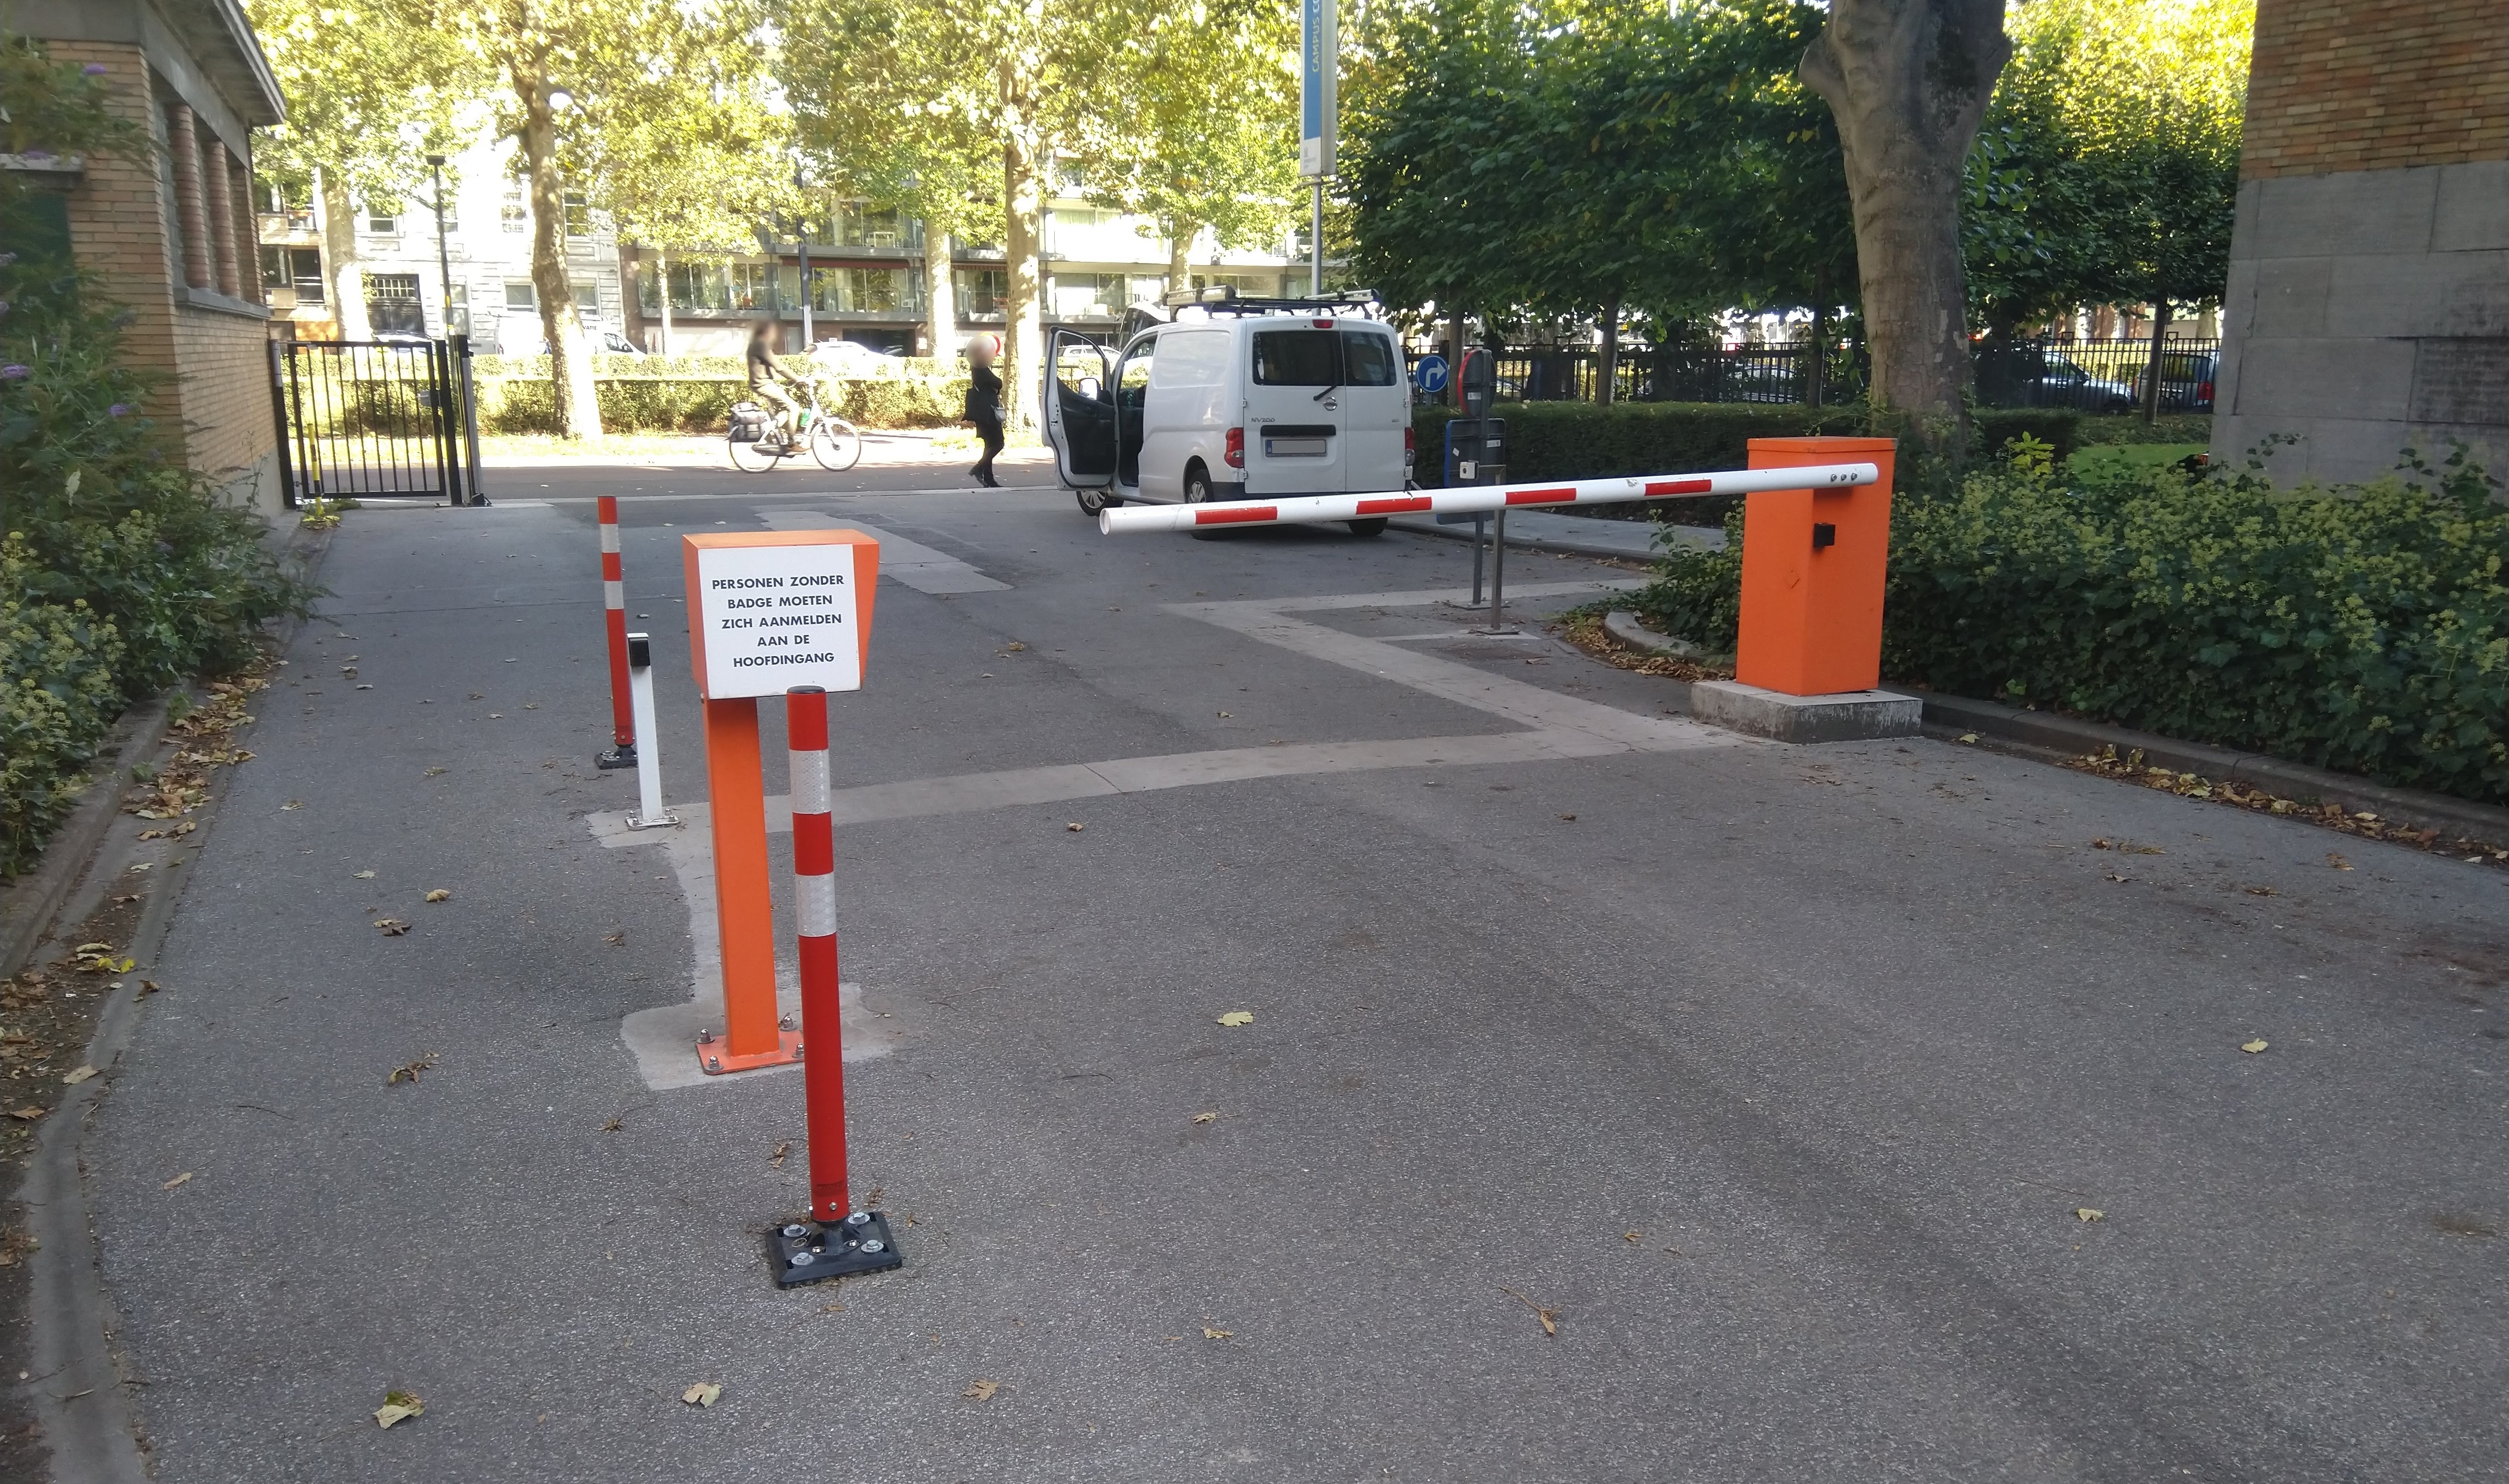
\includegraphics[width=\linewidth]{img/uitgang-coupure.jpg}
	\caption{Uitgang met tokens aan UGent campus Coupure}
\end{figure}

\subsection{Opstelling}
Om de foto's te verkrijgen is gebruik gemaakt van de Raspberry Pi met de PiNoIR camera, deze is op de juiste hoogte van de paal tijdelijk vastgezet worden tezamen met een powerbank. De Raspberry Pi is geconnecteerd met een GSM die als hotspot ingesteld staat, waarop met een SSH verbinding het commando kan worden uitgevoerd om foto's te nemen. Deze foto's worden vervolgens allemaal verzameld en verwerkt.

Figuur \ref{Opstelling} toont de gemaakte opstelling. Deze bevat De Raspberry Pi, de Pi-Cam en een powerbank met een capaciteit van 700mAh.
\begin{figure}[h]
	\centering
	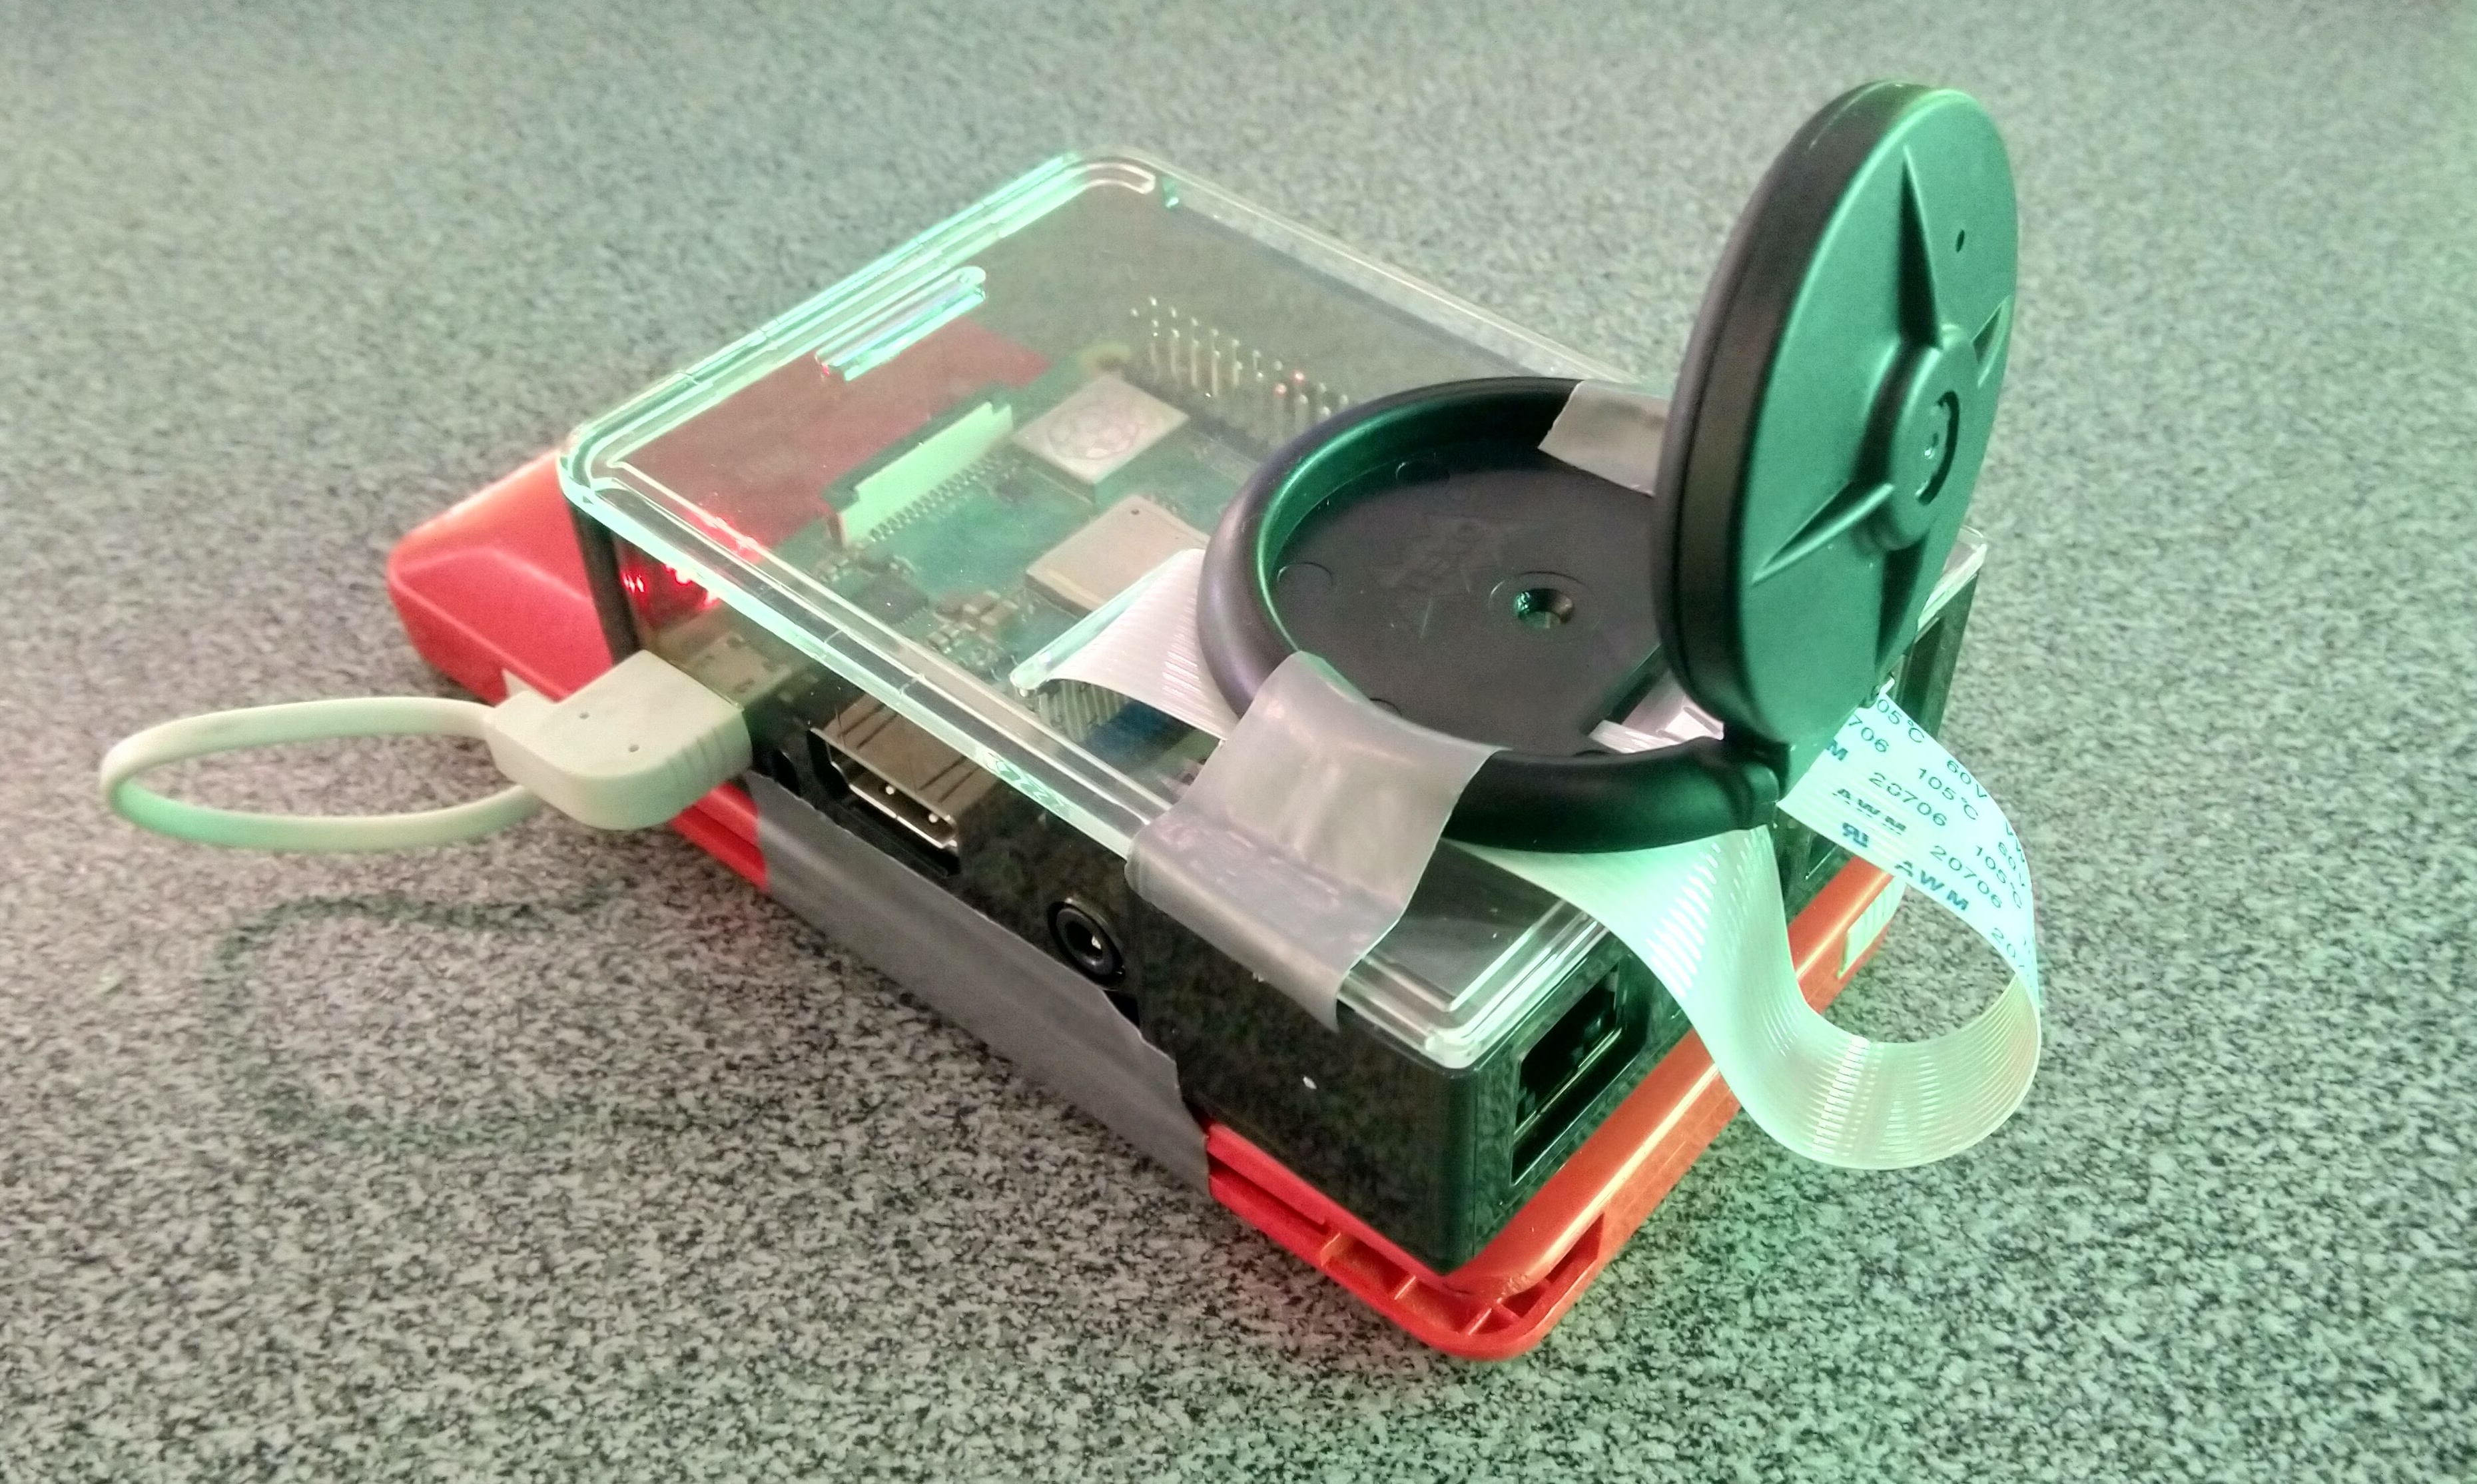
\includegraphics[width=0.5\linewidth]{img/camera.jpg}
	\caption{Opstelling Raspberry Pi met PiCam.}
	\label{Opstelling}
\end{figure}

\section{Verzamelen van de gegevens}
De verzamelde gegevens horen correct te zijn en representatief voor een automatisch geïmplementeerd systeem. Alle uitgevoerde stappen om de gegevens te bekomen zijn in dit onderdeel beschreven tezamen met hun motivaties.

\subsection{Nemen van de foto's}
Het nemen van de foto's is een fysiek onderdeel van dit onderzoek en werd uitgevoerd op de volgende locaties:
\begin{itemize}
	\item Campus Coupure - Uitgang Coupure Links
	\item Campus Coupure - Uitgang Kruisboogstraat
	\item Campus Sterre - Uitgang De Pintelaan
	\item Campus Sterre - Uitgang Galglaan
\end{itemize}

Deze foto's werden gemaakt met de PiNoIR camera verbonden aan de Raspberry Pi m.b.v. het raspistill commando. Per auto die de parking verlaat worden er a.d.h.v. een handmatige trigger 6 foto's gemaakt in een burst van 3 seconden met 500 ms per foto. Dit aan de hand van het raspistill commando:  
\begin{lstlisting}[language=Bash, breaklines=true]
#!/bin/bash

# -t : De timeout waarover foto's genomen worden
# -bm : Gebruik de camera in burst mode, hierdoor moet de camera niet telkens opnieuw focussen tussen iedere genomen foto
# -tl : Tijd tussen iedere foto in burst mode
# --width --height : De resolutie van de bekomen foto's
# --nopreview : schakel de preview uit aangezien er geen monitor verbonden is
raspistill -t 3000 -bm -tl 500 --width 1280 --height 720 --nopreview
-o `date +%d%m%Y_%H%M%S`%04d.jpg
\end{lstlisting}

\subsubsection{Triggering van de camera}
De camera zelf werd in dit onderzoek handmatig getriggerd aangezien een implementatie opstellen voor automatische triggering niet paste binnen het tijdsschema van dit onderzoek.

In een werkelijke implementatie zou deze triggering mogelijk zijn a.d.h.v. software dat de beelden van de Raspberry Pi bekijkt en hierop bewegingsdetectie uitvoert. Een voorbeeld hiervan is de 'motion' package die hiervoor een open-source implementatie geeft.

\subsection{Tijdstippen van de genomen foto's}
In tabel \ref{tab:fototijdstippen} zijn alle momenten genoteerd dat er fysiek foto's verzameld werden. Deze zijn telkens verworven in de vroege namiddag aangezien er op deze momenten nog steeds daglicht is en mensen beginnen te vertrekken van de Campussen. Enkel op de Coupure Links is er later geprobeerd data te verzamelen omdat er overdag bijna geen auto's vertrokken.
\begin{table}[h!]
\centering
\begin{tabular}{l|l|l|l|l}
	Datum 		& Begin & Eind	& Locatie	& Aantal foto's \\ \hline
	06/11/2019	& 11u45 & 12u46	& Campus Coupure - Uitgang Kruisboogstraat	& 48	\\
	08/11/2019	& 12u15 & 12u29	& Campus Sterre - Uitgang Galglaan	& 17	\\
	08/11/2019	& 12u52 & 13u41	& Campus Sterre - Uitgang De Pintelaan	& 38	\\
	13/11/2019	& 11u36 & 12u08	& Campus Sterre - Uitgang De Pintelaan	& 50	\\
	13/11/2019	& 12u29 & 12u42	& Campus Sterre - Uitgang Galglaan	& 9	\\
	13/11/2019	& 13u48 & 14u35	& Campus Coupure - Uitgang Coupure Links	& 5	\\
	14/11/2019	& 18u05 & 18u55	& Campus Coupure - Uitgang Coupure Links	& 3	\\
	21/11/2019	& 14u08 & 15u11	& Campus Sterre - Uitgang De Pintelaan	& 35	\\
	21/11/2019	& 15u58 & 16u22	& Campus Sterre - Uitgang Galglaan	& 36	\\
	27/11/2019	& 13u42 & 15u03	& Campus Sterre - Uitgang De Pintelaan	& 75	\\
	29/11/2019	& 12u04 & 12u35	& Campus Coupure - Uitgang Kruisboogstraat	& 20	\\
	11/12/2019	& 13u42 & 15u12	& Campus Sterre - Uitgang De Pintelaan	& 64	\\
\end{tabular}
\caption{Tijdstippen wanneer de verwerkte foto's bekomen zijn.}
\label{tab:fototijdstippen}
\end{table}

%Zo bekomen we volgende aantallen van foto's per uitgang:
%\begin{table}[h]
%	\centering
%	\begin{tabular}{l|l}
%		Uitgang	& Aantal foto's \\ \hline
%		Campus Coupure - Uitgang Kruisboogstraat	& 53\\
%		Campus Coupure - Uigang Coupure Links	& 5\\
%		Campus Sterre - Uitgang Galglaan	& 32\\
%		Campus Sterre - Uitgang De Pintelaan, camerahoek rechts	& 38\\
%		Campus Sterre - Uitgang De Pintelaan, camerahoek links	& 50\\
%	\end{tabular}
%\end{table}

\subsection{Incorrecte foto's}
Foto's die te laat of te vroeg werden genomen worden weggelaten. Enkele voorbeelden hiervan zijn te zien in Figuur \ref{fig:badpics}. Vervolgens wordt er per auto maar 1 foto bijgehouden per afstand. Indien er maar 1 afstand aanwezig is op de foto's, wordt deze reeks niet gezien als representatief en zullen de auto's niet verwerkt worden.

\begin{figure}[h!]
	\centering
	\begin{subfigure}[b]{0.45\linewidth}
		\includegraphics[width=\linewidth]{img/slecht/close.jpg}
		\caption{Auto op een onredelijk dichte afstand.}
	\end{subfigure}
	\begin{subfigure}[b]{0.45\linewidth}
		\includegraphics[width=\linewidth]{img/slecht/far.jpg}
		\caption{Auto op een onredelijk verre afstand.}
	\end{subfigure}
	\begin{subfigure}[b]{0.45\linewidth}
		\includegraphics[width=\linewidth]{img/slecht/anderekant.jpg}
		\caption{Auto die de parking niet verlaat.}
	\end{subfigure}
	\caption{Types van foto's die niet werden opgenomen in het onderzoek.}
	\label{fig:badpics}
\end{figure}


In sommige gevallen zijn de foto's allemaal van een veel te verre afstand genomen, dit is niet representatief aangezien een motion detection systeem foto's over een korte afstand kan nemen. In het geval van Figuur \ref{fig:onlyfar} zijn alle afbeeldingen op een verre afstand genomen. Een motion detection systeem zou in dit geval ook foto's genomen kunnen hebben op een dichtere afstand, hierdoor is deze reeks foto's niet representatief en zal ook niet opgenomen worden in het onderzoek.
\begin{figure}[h!]
	\centering
	\begin{subfigure}[b]{0.45\linewidth}
		\includegraphics[width=\linewidth]{img/slecht/onlyfar1.jpg}
	\end{subfigure}
	\begin{subfigure}[b]{0.45\linewidth}
		\includegraphics[width=\linewidth]{img/slecht/onlyfar2.jpg}
	\end{subfigure}
	\begin{subfigure}[b]{0.45\linewidth}
		\includegraphics[width=\linewidth]{img/slecht/onlyfar3.jpg}
	\end{subfigure}
	\caption{Foto's die op een te verre afstand genomen zijn en dus niet representatief zijn.}
	\label{fig:onlyfar}
\end{figure}

\section{Verwerking van gegevens}

Nadat de foto's van een uitgang verzameld zijn, werd op iedere foto nummerplaatdetectie uitgevoerd m.b.v. OpenALPR. Het resultaat van deze detectie werd opgeslagen in een JSON bestand naast de corresponderende afbeelding. Hiervoor werd de volgende bash code gebruikt:

\begin{lstlisting}[language=Bash, breaklines=true]
#!/bin/bash

FILES=$(ls -tr *.jpg)
for fullname in $FILES
do
fname="${fullname%.*}"
alpr -p be -c eu --config alpr.config -j $fullname | jq '.' > "${fname}.json"
echo "processed file ${fname}.json" 
done
\end{lstlisting}

Vervolgens werd alle data van de afbeeldingen verzameld in een algemeen CSV bestand, tezamen met de bekomen nummerplaten van OpenALPR.
\begin{itemize}
	\item \textbf{identifier:} Unieke identifier per auto.
	\item \textbf{file:} De bestandsnaam van de foto.
	\item \textbf{license\_plate:} De 'correcte' nummerplaat, handmatig uit de foto gehaald.
	\item \textbf{result:} De nummerplaat gedetecteerd door OpenALPR.
	\item \textbf{distance:} De afstand van de camera, bestaat uit drie velden, "close", "medium"\ en "far". Close betekent een afstand onder de 3 meter, medium tussen 3 en 5 meter en far betekent verder dan 5 meter.
	\item \textbf{lighting:} De belichting van de nummerplaten, bestaat uit 2 velden, "bright"\ en "very\_bright". Bright betekent dat de nummerplaat duidelijk leesbaar is voor mensen onder normaal daglicht. very\_bright betekent dat deze niet onmiddelijk leesbaar is.
	\item \textbf{location:} De uitgang waar de foto is genomen, bestaat uit "coupure-kruisboogstraat", "coupure-coupurelinks", "sterre-galglaan"\ en "sterre-depintelaan".
\end{itemize}

Ten laatste zijn deze resultaten verwerkt in de statistische taal 'R'. De code voor deze bewerkingen zijn te vinden in bijlage \ref{ch:bijlageperfoto} en bijlage \ref{ch:bijlageperauto}.

\subsection{Kalibratie van de afbeeldingen}
Origineel waren alle resultaten van de nummerplaatdetectie aan de zeer lage kant, aangezien de afbeeldingen nog niet gekalibreerd waren. Maar met de tools beschreven in onderdeel \ref{alprcalib}, was het mogelijk om een algemene transformatie op de afbeeldingen uit te voeren.
\begin{figure}[h!]
	\centering
	\begin{subfigure}[b]{0.4\linewidth}
		\includegraphics[width=\linewidth]{img/calibration/pre-calibrate.png}
		\caption{Niet-gekalibreerde afbeelding}
	\end{subfigure}
	\begin{subfigure}[b]{0.4\linewidth}
		\includegraphics[width=\linewidth]{img/calibration/calibrate-cut.png}
		\caption{Gekalibreerde afbeelding}
	\end{subfigure}
	\label{fig:calibration}
	\caption{Calibratie van afbeeldingen met behulp van openalpr-utils-calibrate.}
\end{figure}

Het verschil in de bekomen resultaten is duidelijk merkbaar. In tabel \ref{tab:kalibratiealpr} worden de resultaten per foto vergeleken waarbij wel gekalibreerd en niet-gekalibreerd is. De resultaten stijgen van een 41.9\% naar een 79.0\%. Kalibratie is dus wellicht een noodzakelijk onderdeel van een geslaagde implementatie.
\begin{table}[h!]
	\centering
	\begin{tabular}{l|l|l|l|l}
		 		& Incorrect & Correct & Totaal & Ratio	\\ \hline
		Niet-gekalibreerd	& 36 & 26 & 62 & 41.9\%	\\
		Gekalibreerd	& 13 & 49 & 62 & 79.0\%\\
	\end{tabular}
\caption{Verschil in nauwkeurigheid per foto door de kalibratie van OpenALPR.}
\label{tab:kalibratiealpr}
\end{table}

\subsection{Patroon matching van nummerplaten}
Nummerplaten kunnen soms foutief gedetecteerd worden door letters en nummers die op elkaar lijken. Zo is er maar een klein verschil tussen de O, 0 en Q. 
Hierdoor kan het zijn dat een nummerplaat zoals 1-NOP-123 gelezen wordt als 1-N0P-123. In de gevallen dat deze de structuur van de reeksen tekens in de nummerplaten verhinderen, kunnen deze gemakkelijk opgelost worden door gebruik van OpenALPR's patroon matching.

Wat patroon matching doet is zoals de naam zegt; het controleren of een bekomen nummerplaat voldoet aan een bepaald patroon. In België en Nederland zijn deze sinds 2010 een 1 met 3 letters en 3 cijfers.

\section{Resultaten}

\subsection{Campus Sterre - Uitgang Galglaan}

De uitgang aan de Galglaan is één van de twee uitgangen op de campus Sterre. De uitgang ligt naast de straat Galglaan en heeft twee inrijrichtingen. Deze locatie is aangeduid in figuur \ref{fig:satteliet-galglaan}.
\begin{figure}[h!]
	\centering
	\includegraphics[width=0.8\linewidth]{img/res-galglaan/satteliet-galglaan.png}
	\caption{Satellietafbeelding van de Campus Sterre - Uitgang Galglaan. De uitgang zelf is aangeduid met een rode cirkel. De uitrijrichting met een rode pijl. \autocite{ugent2019google}}
	\label{fig:satteliet-galglaan}
	\centering
	\includegraphics[width=0.8\linewidth]{img/res-galglaan/galg.jpg}
	\caption{Close-up van de uitgang aan Campus Sterre - Uitgang Galglaan. De cameralocatie is aangeduid met een rode cirkel en de uitrijrichting met een rode pijl.}
	\label{fig:galglaan}
\end{figure}

Aan de hand van de informatie bekomen in hoofdstuk \ref{ch:maatregelenanpr}, werd er besloten om de camera op de metalen constructie van de hefboom te plaatsen. Deze is te zien in figuur \ref{fig:galglaan} en is gekozen op basis van de volgende standpunten:
\begin{itemize}
	\item De hoogte van de metalen constructie is hoog genoeg om direct licht van koplampen te verhelpen.
	\item Vanuit deze locatie is een grote afstand van de rijbaan zichtbaar van aankomende voertuigen. Dit geeft het systeem een grotere kans om een auto te identificeren.
	\item De camera op de metalen constructie monteren is een voordeel op vlak van implementatiekosten. Bekabeling is reeds aanwezig in de kast en geen extra paal moet geplaatst worden om de camera te monteren.
\end{itemize}

\paragraph{Resultaat}
Met deze gekozen cameraplaatsing zijn vervolgens 23 verschillende voertuigen verwerkt en zijn de volgende resultaten bekomen:
\begin{table}[h!]
	\centering
	\begin{tabular}{l|l|l|l|l}
\textbf{ANPR nauwkeurigheid: Galglaan} & Incorrect & Correct & Totaal & Ratio	\\ \hline
Per individuele foto 	& 13 & 49	& 62	& 79.0\%\\
Per auto				& 1 & 22	& 23 	& 95.7\%\\
\end{tabular}
\caption{Resultaten van OpenALPR aan Campus Sterre - Uitgang Galglaan.}
\label{tab:anprgalglaan}
\end{table}

Deze resultaten zijn volgens de originele verwachtingen van een resultaat rond de 95\%. Deze foutmarge is laag genoeg om te kunnen besluiten dat nummerplaatdetectie aan deze uitgang mogelijk is in normaal belichte omstandigheden. Mogelijks kan dit resultaat verbeterd worden door het verhogen van de resolutie van de genomen afbeeldingen of het upgraden van OpenALPR naar de commerciële versie.

\paragraph{Fouten}
De enkele foutieve wagen, getoond in figuur \ref{foutiefgalglaan}, heeft geen opvallende verschillen dan de andere wel-gedetecteerde wagens. Qua positie, kwaliteit, focus is hij identiek. We kunnen hierdoor veronderstellen dat deze fout komt door de accuraatheid van OpenALPR zelf, of aan de resolutie van de afbeeldingen.
\begin{figure}[h!]
	\centering
	\includegraphics[width=0.5\linewidth]{img/res-galglaan/galg1.jpg}
	\caption{Niet-gedetecteerde nummerplaat aan Campus Sterre - Galglaan. Enkele karakters van de nummerplaat zijn onleesbaar gemaakt uit privacy van de bestuurder.}
	\label{foutiefgalglaan}
\end{figure}

\subsection{Campus Sterre - Uitgang De Pintelaan}
De uitgang op de Campus Sterre aan de De Pintelaan is de hoofduitgang van UGent Campus Sterre en was een uitdaging om correct te configureren. Deze is verbonden met drie straten die enkele grote parkings verbinden, bijgevolg wordt deze het meest gebruikt van alle uitgangen. Het is dan ook belangrijk dat hier een goede detectie is.

Door de vele verbindingen is het mogelijk om de parking op allerlei manieren te bereiken, deze zijn te zien op figuur \ref{fig:satellietdepintelaan}. Dit is op zich geen probleem, maar hierdoor moet de nummerplaatdetectie wel in een groot aantal oriëntaties werken.

Aangezien aan deze uitgang niet direct een optimale camerahoek gevonden was, worden in de volgende onderdelen de geteste camerahoeken beschreven tezamen met hun resultaten. Deze camerahoeken zijn aangeduid met cijfers in figuur \ref{fig:satellietdepintelaan}.

\begin{figure}[h!]
	\centering
	\includegraphics[width=\linewidth]{img/satellietdepintelaan.png}
	\caption{Satellietafbeelding van de Campus Sterre - Uitgang De Pintelaan met aangeduide routes en cameralocaties. \autocite{ugent2019google}}
	\label{fig:satellietdepintelaan}
\end{figure}

\subsubsection{Positie rechts van de hefboom}
In een eerste poging tot een goede detectie werd de camera op de metalen constructie van de hefboom geplaatst, wat op de uitgang van de Galglaan al degelijke resultaten opleverde. Spijtig genoeg was deze locatie duidelijk niet geschikt, de zon speelde een grote invloed op de afbeeldingen en ook de vele inrijrichtingen maakten dit moeilijk.

Deze plaatsing van de camera is aangeduid op afbeelding \ref{fig:satellietdepintelaan} als punt 1. Figuur \ref{fig:plaatsingdepintelaanorigineel} verduidelijkt de specifieke plaatsing van de camera zelf.

\begin{figure}[h!]
	\centering
	\includegraphics[width=0.8\linewidth]{img/depintelaanorigineel.jpg}
	\caption{Cameraplaatsing aan de rechterkant van de hefboom op Campus Sterre - De Pintelaan. De locatie van de camera is aangeduid met een rode cirkel. De uitrijrichting is van links naar rechts}
	\label{fig:plaatsingdepintelaanorigineel}
\end{figure}

\begin{table}[h!]
	\centering
	\begin{tabular}{l|l|l|l|l}
		\textbf{ANPR nauwkeurigheid: De Pintelaan, rechts} & Incorrect & Correct & Totaal & Ratio	\\ \hline
		Per individuele foto 	& 43	& 30	& 73 & 41.1\%\\
		Per auto				& 8	& 17 	& 25 & 68.0\%\\
	\end{tabular}
\caption{Resultaten van OpenALPR aan Campus Sterre - Uitgang Depintelaan, camerahoek 1.}
\label{tab:alprdepintelaan1}
\end{table}

De eerste resultaten aan deze uitgang waren niet denderend, indien 32\% van de bezoekers terug moeten keren om toch een token te halen doet nummerplaatdetectie meer kwaad dan goed. Na het inspecteren van de foutieve afbeelding werd duidelijk dat vele voertuigen 's middags een grote interferentie van het zonlicht hadden. Wanneer de zon hoog staat reflecteerde het zonlicht via de nummerplaat recht in de camera, wat het contrast van de tekst op de nummerplaat in grote mate verminderde en de detectie onmogelijk maakte. Hieruit kon er afgeleid worden dat deze specifieke cameraplaatsing niet geschikt is voor de uitgang en een andere camerahoek gezocht moest worden. 

Een voorbeeld van deze interferentie is te zien op Figuur \ref{SterreZonlicht}. Deze afbeelding is niet bewerkt, de nummerplaat is gewoonweg helemaal niet zichtbaar door de reflectie van het zonlicht.
\begin{figure}[h!]
	\centering
	\includegraphics[width=0.8\linewidth]{img/sterre2zon.jpg}
	\caption{Interferentie van zonlicht op de parking van Campus Sterre - De Pintelaan, camerahoek 1.}
	\label{SterreZonlicht}
\end{figure}

\subsubsection{Positie links van de hefboom}
In een poging om de invloed van de zon tegen te gaan is geprobeerd om de camera aan de linkerkant van de slagboom te zetten, maar ook op deze positie maakte de zon de nummerplaten in vele gevallen minder leesbaar, bijkomend gaf de camerahoek zelf enkele nadelen. Door de vele inrijrichtingen van de auto, aangeduid op figuur \ref{fig:satellietdepintelaan}, waren een groot deel van de nummerplaten helemaal niet zichtbaar. Enkele voorbeelden hiervan zijn te zien in figuur \ref{fig:sterre-links}, Auto's die van links komen hun nummerplaten staan te schuin om soms zelfs duidelijk met het oog te kunnen lezen.

\begin{figure}[h!]
	\centering
	\begin{subfigure}[b]{0.4\linewidth}
		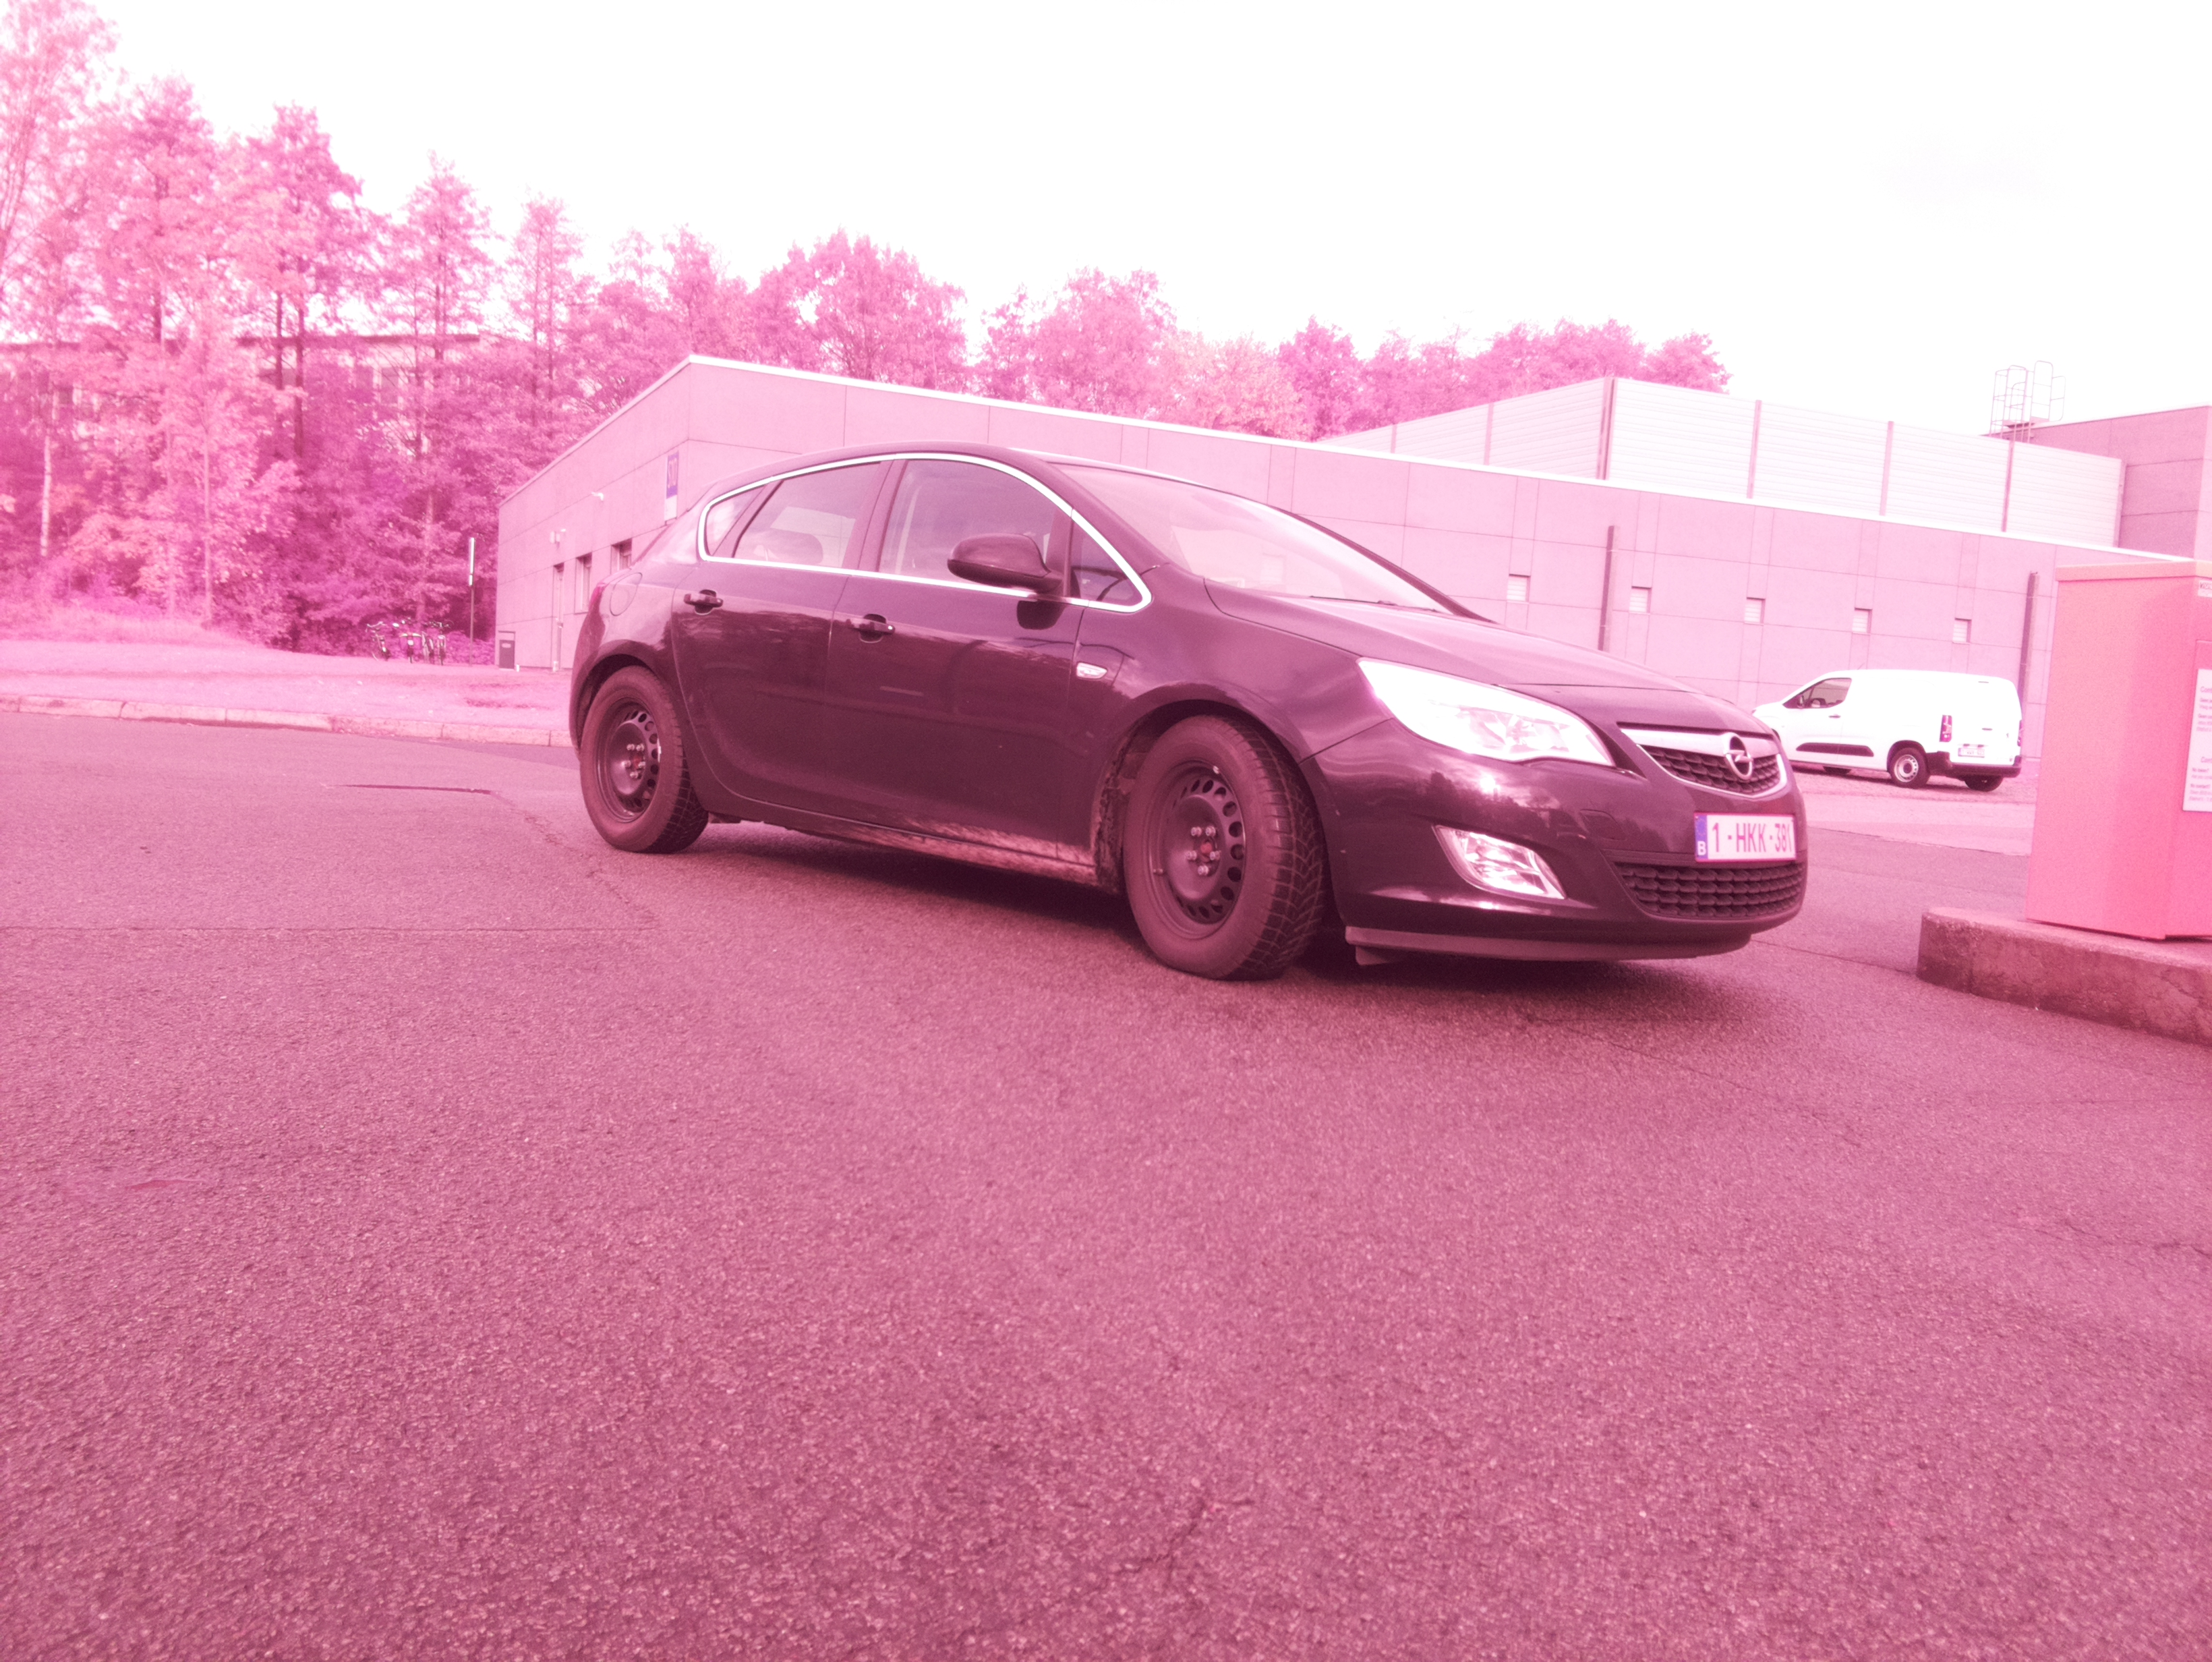
\includegraphics[width=\linewidth]{img/sterlinks/sterrelinks1.jpg}
	\end{subfigure}
	\begin{subfigure}[b]{0.4\linewidth}
		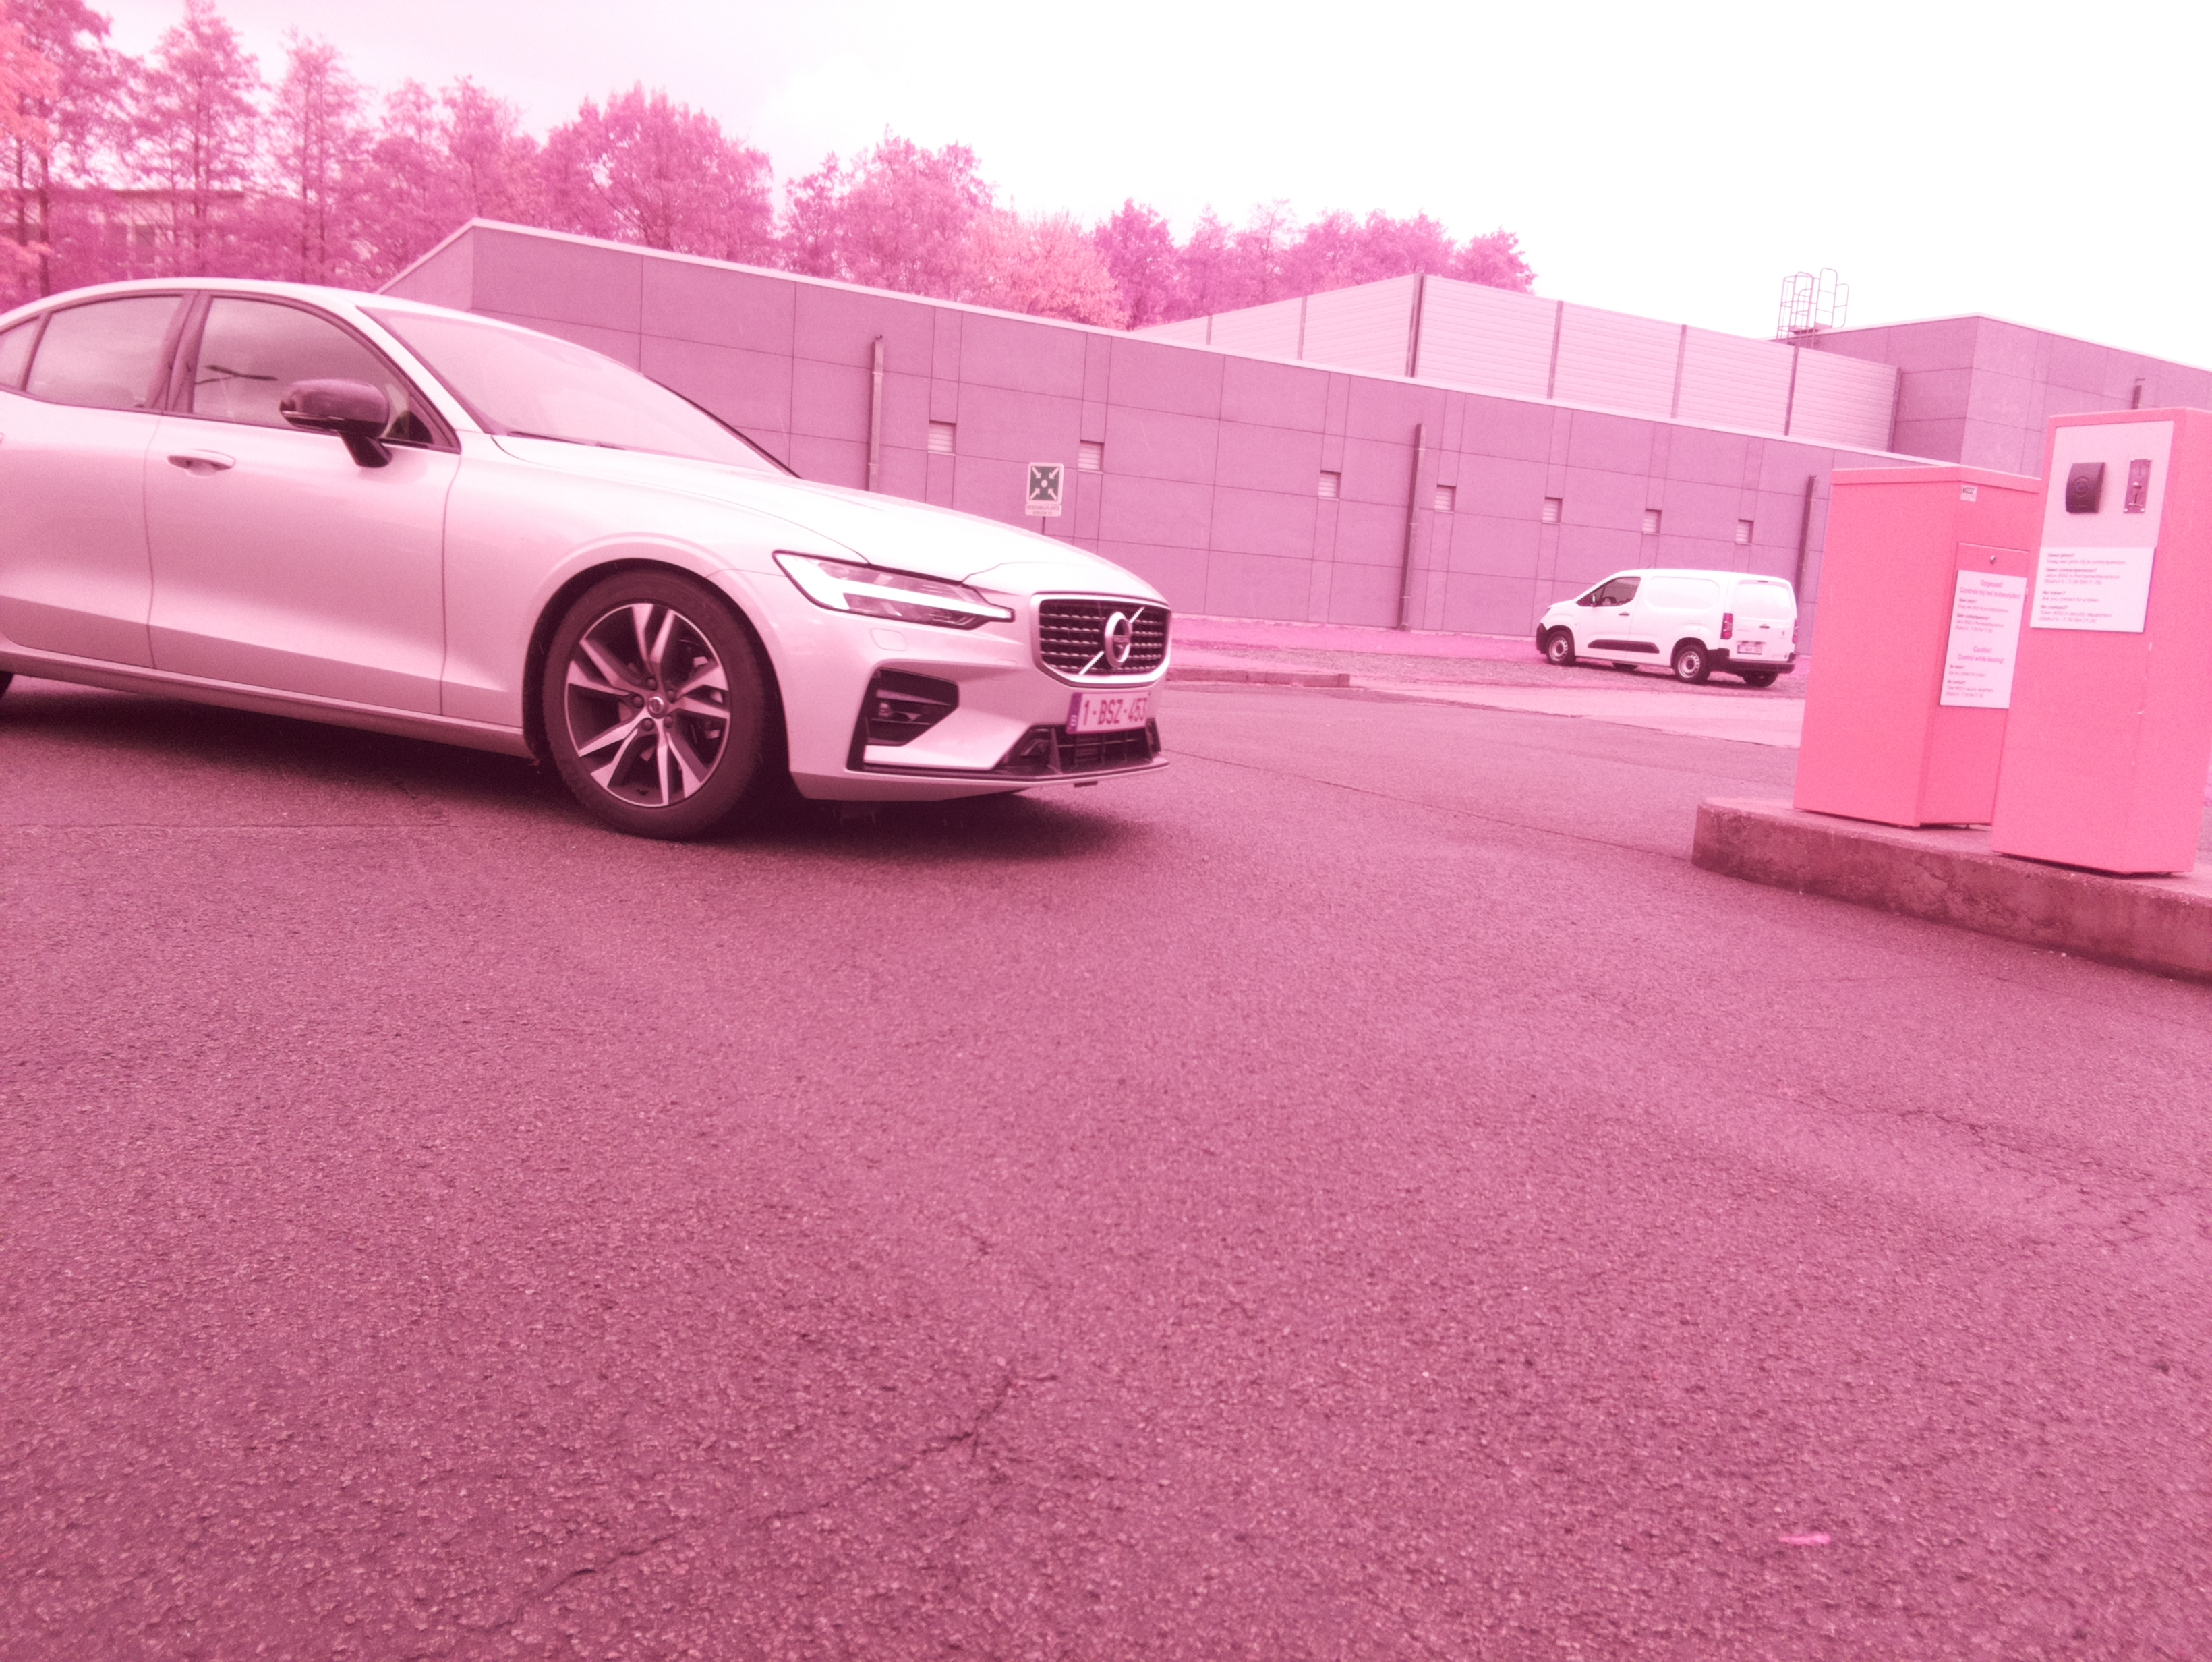
\includegraphics[width=\linewidth]{img/sterlinks/sterlinks2.jpg}
	\end{subfigure}
	\caption{Moeilijk te detecteren nummerplaten door scherpe camerahoek.}
	\label{fig:sterre-links}
\end{figure}

Hierdoor verkrijgen we volgende resultaten:
\begin{table}[h!]
	\centering
	\begin{tabular}{l|l|l|l|l}
		\textbf{ANPR nauwkeurigheid: De Pintelaan, links} & Totaal & Incorrect & Correct & Ratio	\\ \hline
		Per individuele foto 	& 50 & 31	& 19	& 38.0\%\\
		Per auto				& 17 & 8	& 9 	& 52.9\%\\
	\end{tabular}
\caption{Resultaten van OpenALPR aan Campus Sterre - Uitgang De Pintelaan, camerahoek 2.}
\label{tab:alprdepintelaan2}
\end{table}

Met een slechter resultaat dan de vorige positie en net meer dan de helft van de auto's correct te kunnen detecteren, kunnen we besluiten dat deze positie geen oplossing is.

\subsubsection{Positie achteraan de uitgang}
Als derde optie is er getest op de mogelijkheid om van een verdere locatie foto's te nemen aan de hand van een statief om de camera op een geschikte hoogte te houden. Dit is aangetoond op figuur \ref{plaatsingdepintelaan}. Door de camera naar achteren te zetten zorgen de inrijrichtingen voor geen problemen meer aangezien de wagens allemaal op dezelfde plaats kunnen gefotografeerd worden. Verder is er geen storing meer van het zonlicht omdat de camera hoog staat en naar omlaag is gericht.

Deze positie is ongeveer drie meter naar achteren van de linkerkant van de hefboom, dit zodat de invalshoek van de camera zo klein mogelijk blijft. De hoogte van de camera is 1,5 meter hoog, wat hoog genoeg was om de invloed van het zonlicht weg te werken.
\begin{figure}[h!]
	\centering
	\includegraphics[width=0.8\linewidth]{img/depintelaanstatief.jpg}
	\caption{Cameraplaatsing met statief op Campus Sterre - De Pintelaan.}
	\label{plaatsingdepintelaan}
\end{figure}

Volgende resultaten zijn bekomen aan de uitgang:
\begin{table}[h!]
	\centering
	\begin{tabular}{l|l|l|l|l}
		\textbf{ANPR nauwkeurigheid: De Pintelaan, achteraan} & Totaal & Incorrect & Correct & Ratio	\\ \hline
		Per individuele foto 	& 75 & 35	& 40	& 53.3\%\\
		Per auto				& 24 & 6	& 18 	& 75.0\%\\
	\end{tabular}
\caption{Resultaten van OpenALPR aan Campus Sterre - Uitgang De Pintelaan, camerahoek 3.}
\label{tab:alprdepintelaan3}
\end{table}

Deze locatie is een verbetering t.o.v. de vorige posities. Allereerst staan alle auto's op dezelfde locatie ongeacht van inrijrichting. Dit maakt de configuratie van OpenALPR een pak efficiënter.

Ondanks deze voordelen is de nauwkeurigheid niet hoog genoeg en werden er toch 6 auto's niet gedetecteerd . Na deze foto's na te gaan is het duidelijk dat dit komt door de grote afstand en bijgevolg lagere resolutie van de nummerplaten. Een voorbeeld hiervan is te zien op figuur \ref{fig:lowressterre}.

Verder werd één voertuig niet gedetecteerd, niet door de lage resolutie, maar door de hoogte van de slagboom. Deze vrachtwagen's nummerplaat is te hoog aan het voertuig gemonteerd waardoor de slagboom ervoor staat op de foto. Dit is te zien in figuur \ref{fig:slagboomster}. Deze situatie is wellicht uitzonderlijk. Alle andere auto's hun nummerplaten zitten ruim onder de slagboom.

\begin{figure}[h!]
	\centering
	\begin{subfigure}[b]{0.49\linewidth}
		\includegraphics[width=\linewidth]{img/sterachter/sterachter1.jpg}
	\end{subfigure}
	\begin{subfigure}[b]{0.49\linewidth}
		\includegraphics[width=\linewidth]{img/sterachter/sterachter2.png}
	\end{subfigure}
	\caption{Moeilijk te detecteren nummerplaten door een te lage resolutie. Enkele karakters zijn onduidelijk gemaakt uit privacy van de bestuurder.}
	\label{fig:lowressterre}
\end{figure}

\begin{figure}[h!]
	\centering
	\begin{subfigure}[b]{0.99\linewidth}
		\includegraphics[width=\linewidth]{img/sterachter/sterachter3.jpg}
	\end{subfigure}
	\caption{Niet te detecteren nummerplaat omwille van slagboom die het zicht verhindert.}
	\label{fig:slagboomster}
\end{figure}

\subsubsection{Positie achteraan de uitgang - hoge resolutie}
Ten laatste is de steekproef op de vorige positie opnieuw uitgevoerd. De nauwkeurigheid van de PiNoIR camera biedt echter een veel hogere resolutie aan dan dat zij origineel ingesteld waren. Dit maakte het mogelijk om softwarematig in te zoomen op de foto's met een betere kwaliteit. In afbeelding \ref{fig:ressterrecomparison} is dit verschil in kwaliteit van de foto's duidelijk te zien.

\begin{figure}[h!]
	\centering
	\begin{subfigure}[b]{0.49\linewidth}
		\includegraphics[width=\linewidth]{img/sterachter/sterachter2.png}
		\caption{Originele kwaliteit}
	\end{subfigure}
	\begin{subfigure}[b]{0.49\linewidth}
		\includegraphics[width=\linewidth]{img/sterachter/hressmall2.png}
		\caption{Verhoogde kwaliteit}
	\end{subfigure}
	\caption{Verhoogde nauwkeurigheid door het inzoomen van de camera.}
	\label{fig:ressterrecomparison}
\end{figure}

Na de camera vervolgens opnieuw te kalibreren zijn volgende resultaten bekomen:
\begin{table}[h!]
	\centering
	\begin{tabular}{l|l|l|l|l}
		\textbf{ANPR nauwkeurigheid: De Pintelaan, achteraan} & Totaal & Incorrect & Correct & Ratio	\\ \hline
		Per individuele foto 	& 64 & 19	& 45	& 70.3\%\\
		Per auto				& 26 & 2	& 24 	& 92.0\%\\
	\end{tabular}
\caption{Resultaten van OpenALPR aan Campus Sterre - Uitgang De Pintelaan, camerahoek 3 met hogere resolutie.}
\label{tab:alprdepintelaan4}
\end{table}

Deze zijn een enorm verschil met het vorig resultaat van 75\% en bieden een haalbare oplossing voor de uitgang van de De Pintelaan.

\paragraph{Nadelen}
Indien een camera op deze locatie moet gezet worden zullen er enkele maatregelingen nodig zijn om de camera te plaatsen en van stroom te voorzien. Een paal zou in de straat moeten vastgezet worden en een reeks kabels voor stroom en data moeten naar de metalen constructie van de hefboom lopen. Dit vraagt een redelijke hoeveelheid meer werk en kosten dan een systeem dat op de behuizing zelf staat.

\paragraph{Verbeteringen}
De camera is niet direct te hoog geplaatst, dit was uit voorzorg dat de hefboom van de toegang het beeld van de nummerplaten overlapt. Na de foto's te analyseren bleek het toch dat er nog ruim veel plaats was om de camera hoger te zetten. Dit is een vereiste om mogelijke voorbijgangers te beletten van vandalisme. Er wordt verondersteld dat het verhogen van de camera geen direct negatieve invloed op de resultaten zal hebben, dit zolang de kalibratie opnieuw wordt uitgevoerd.

\subsection{Campus Coupure - Uitgang Kruisboogstraat}

De uitgang aan de Kruisboogstraat is de hoofduitgang van de Campus Coupure. Deze uitgang is zeer dichtbij gelegen met 3 van de 4 parkings van de campus, en heeft dus een redelijk hoog aantal auto's die deze gebruikt. Deze locatie is te zien in figuur \ref{fig:sat-kruisboog}, aangeduid met een rode cirkel. Een close-up van de uitgang is te zien in figuur \ref{fig:Kruisboog-uitgang}. 

\begin{figure}[h!]
	\centering
	\includegraphics[width=\linewidth]{img/kruisboog/sateliet-kruisboog.jpg}
	\caption{Satellietafbeelding van de uitgang aan de Kruisboogstraat. De uitgang zelf is aangeduid met een rode cirkel. \autocite{ugent2019google}}
	\label{fig:sat-kruisboog}
\end{figure}

\begin{figure}[h!]
	\centering
	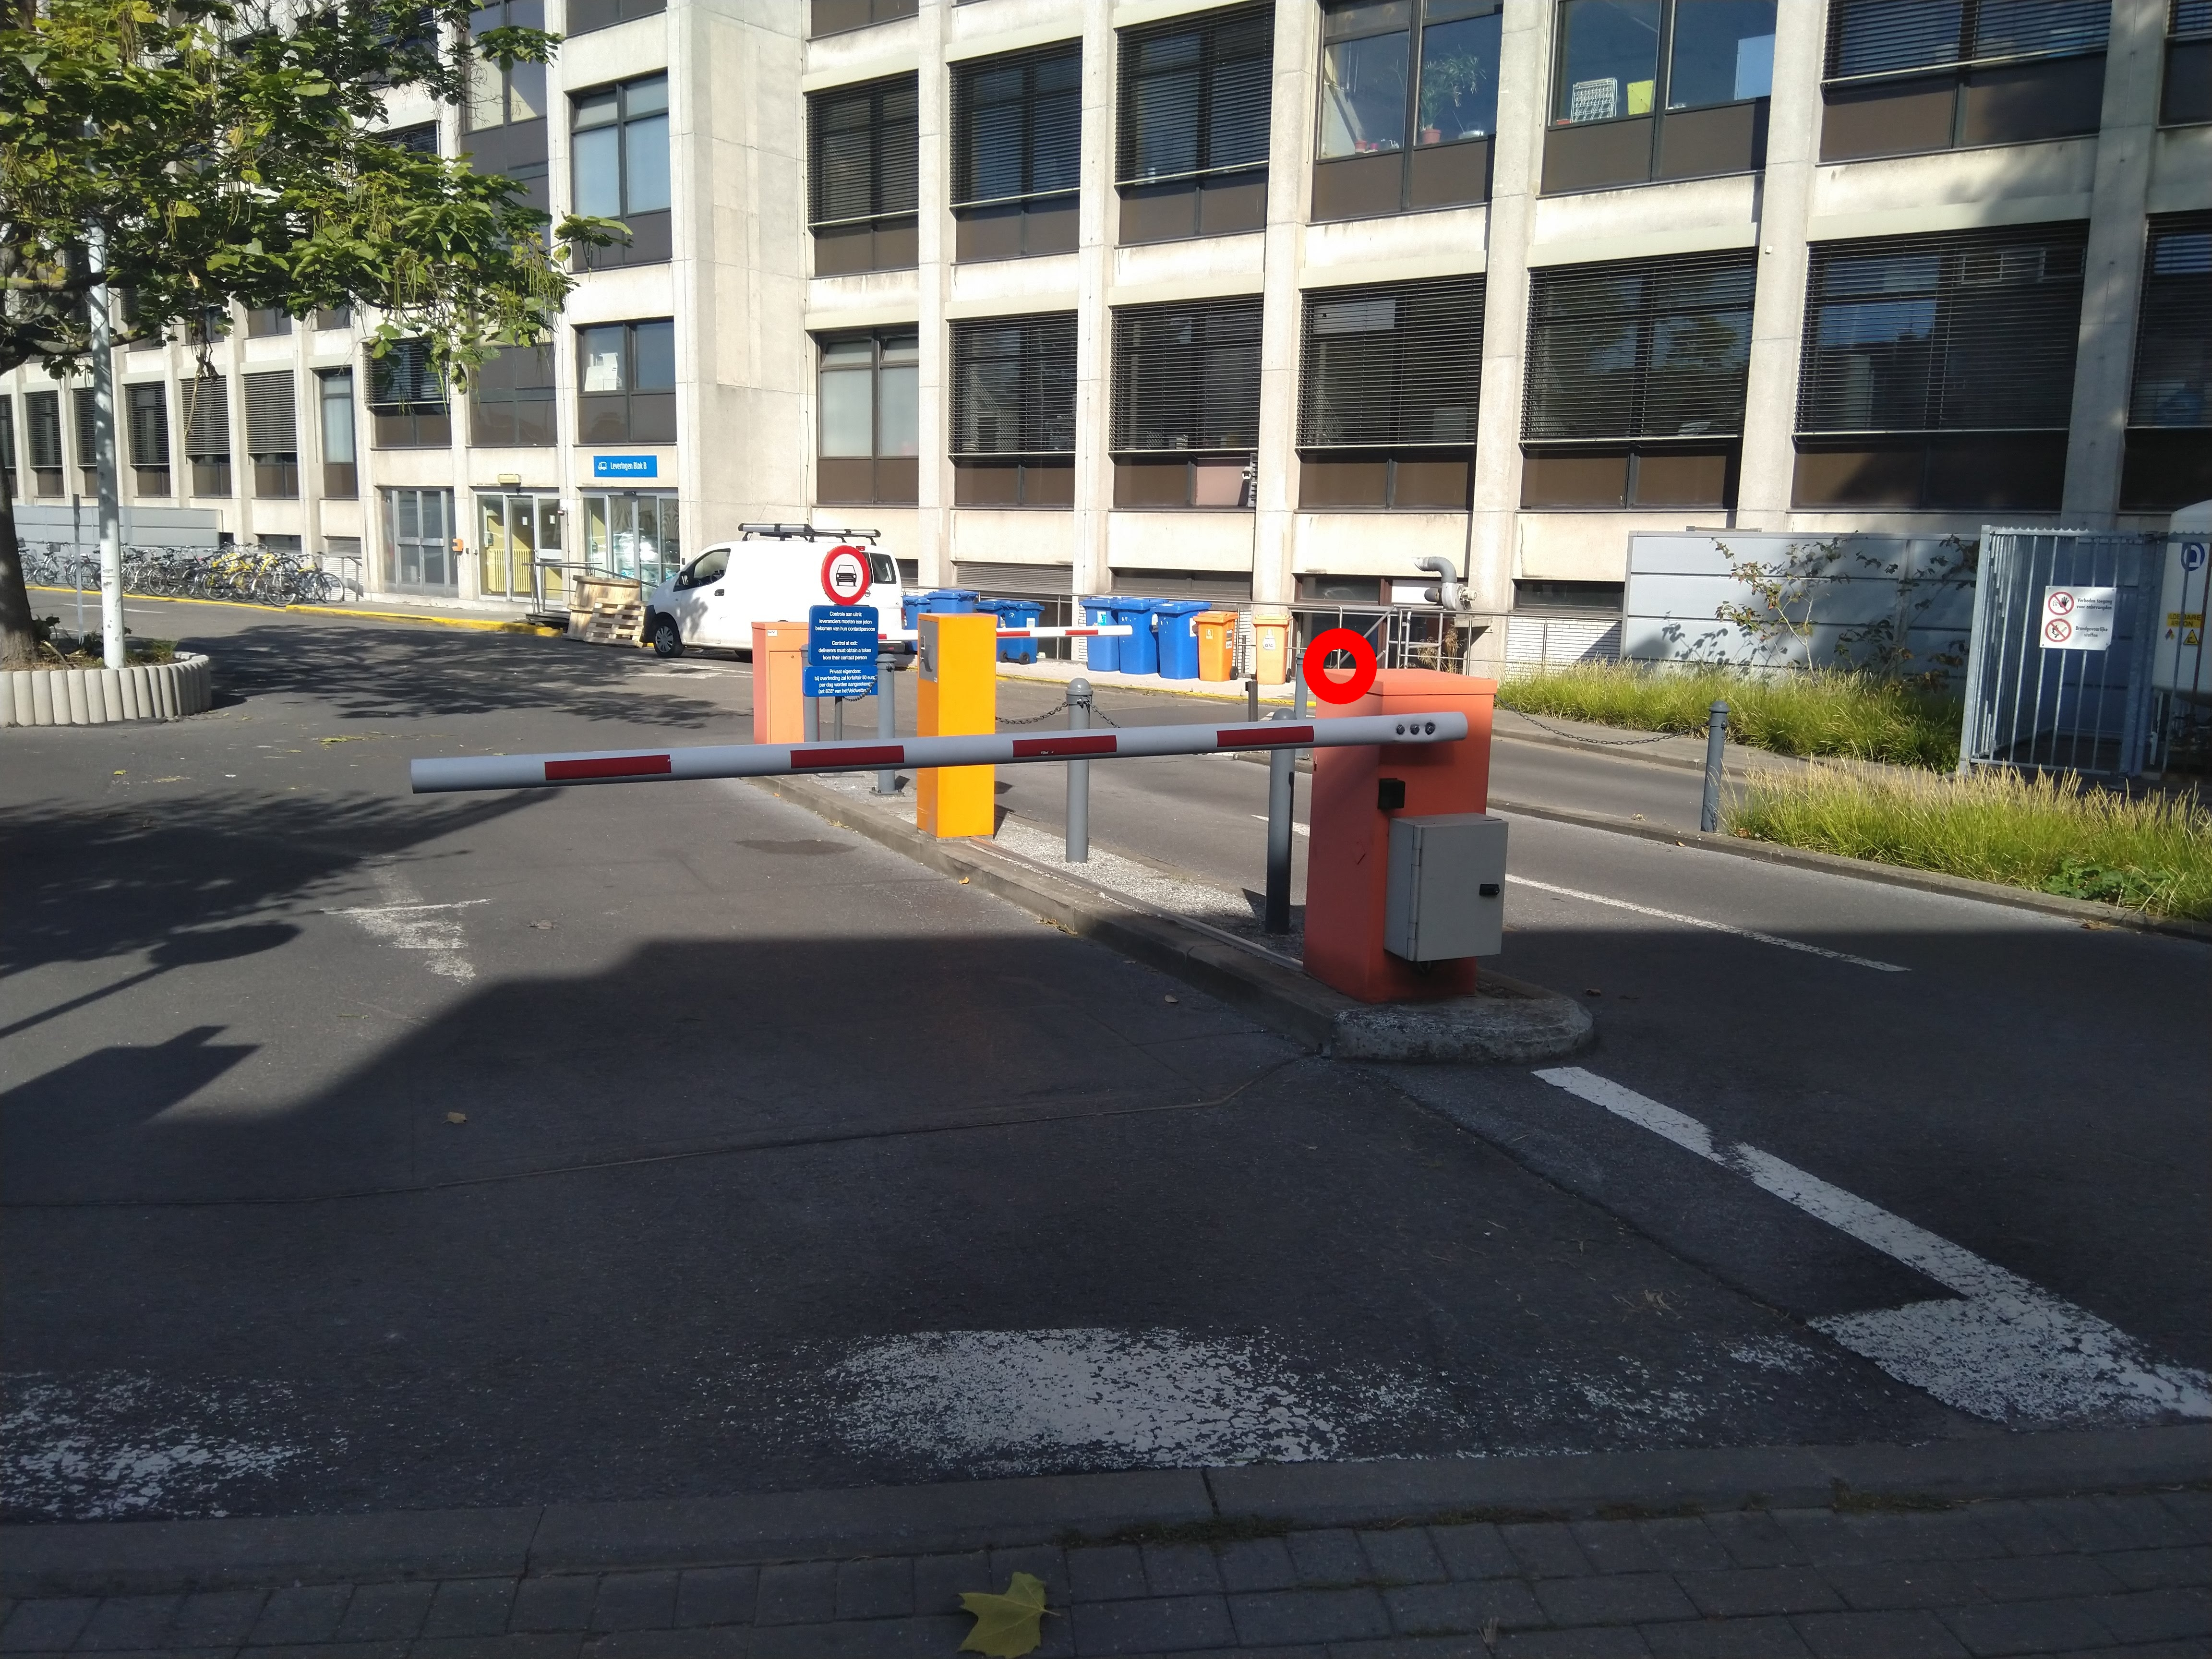
\includegraphics[width=0.9\linewidth]{img/kruisboog/kruisboog-uitgang.jpg}
	\caption{Close-up foto van de uitgang aan de Kruisboogstraat. De locatie van de camera is aangeduid met een rode cirkel.}
	\label{fig:Kruisboog-uitgang}
\end{figure}

Er werd gekozen om de camera op de metalen constructie van de hefboom te plaatsen aangezien deze een brede kijk geeft op alle mogelijke inrijrichtingen, wat te zien is in figuur \ref{fig:Kruisboog}, maar ook omdat deze bij een werkelijke implementatie gemakkelijk te monteren zou zijn. Dit omdat enkele bekabelingen reeds aanwezig is in de montage van de hefboom.

\begin{figure}[h!]
	\centering
	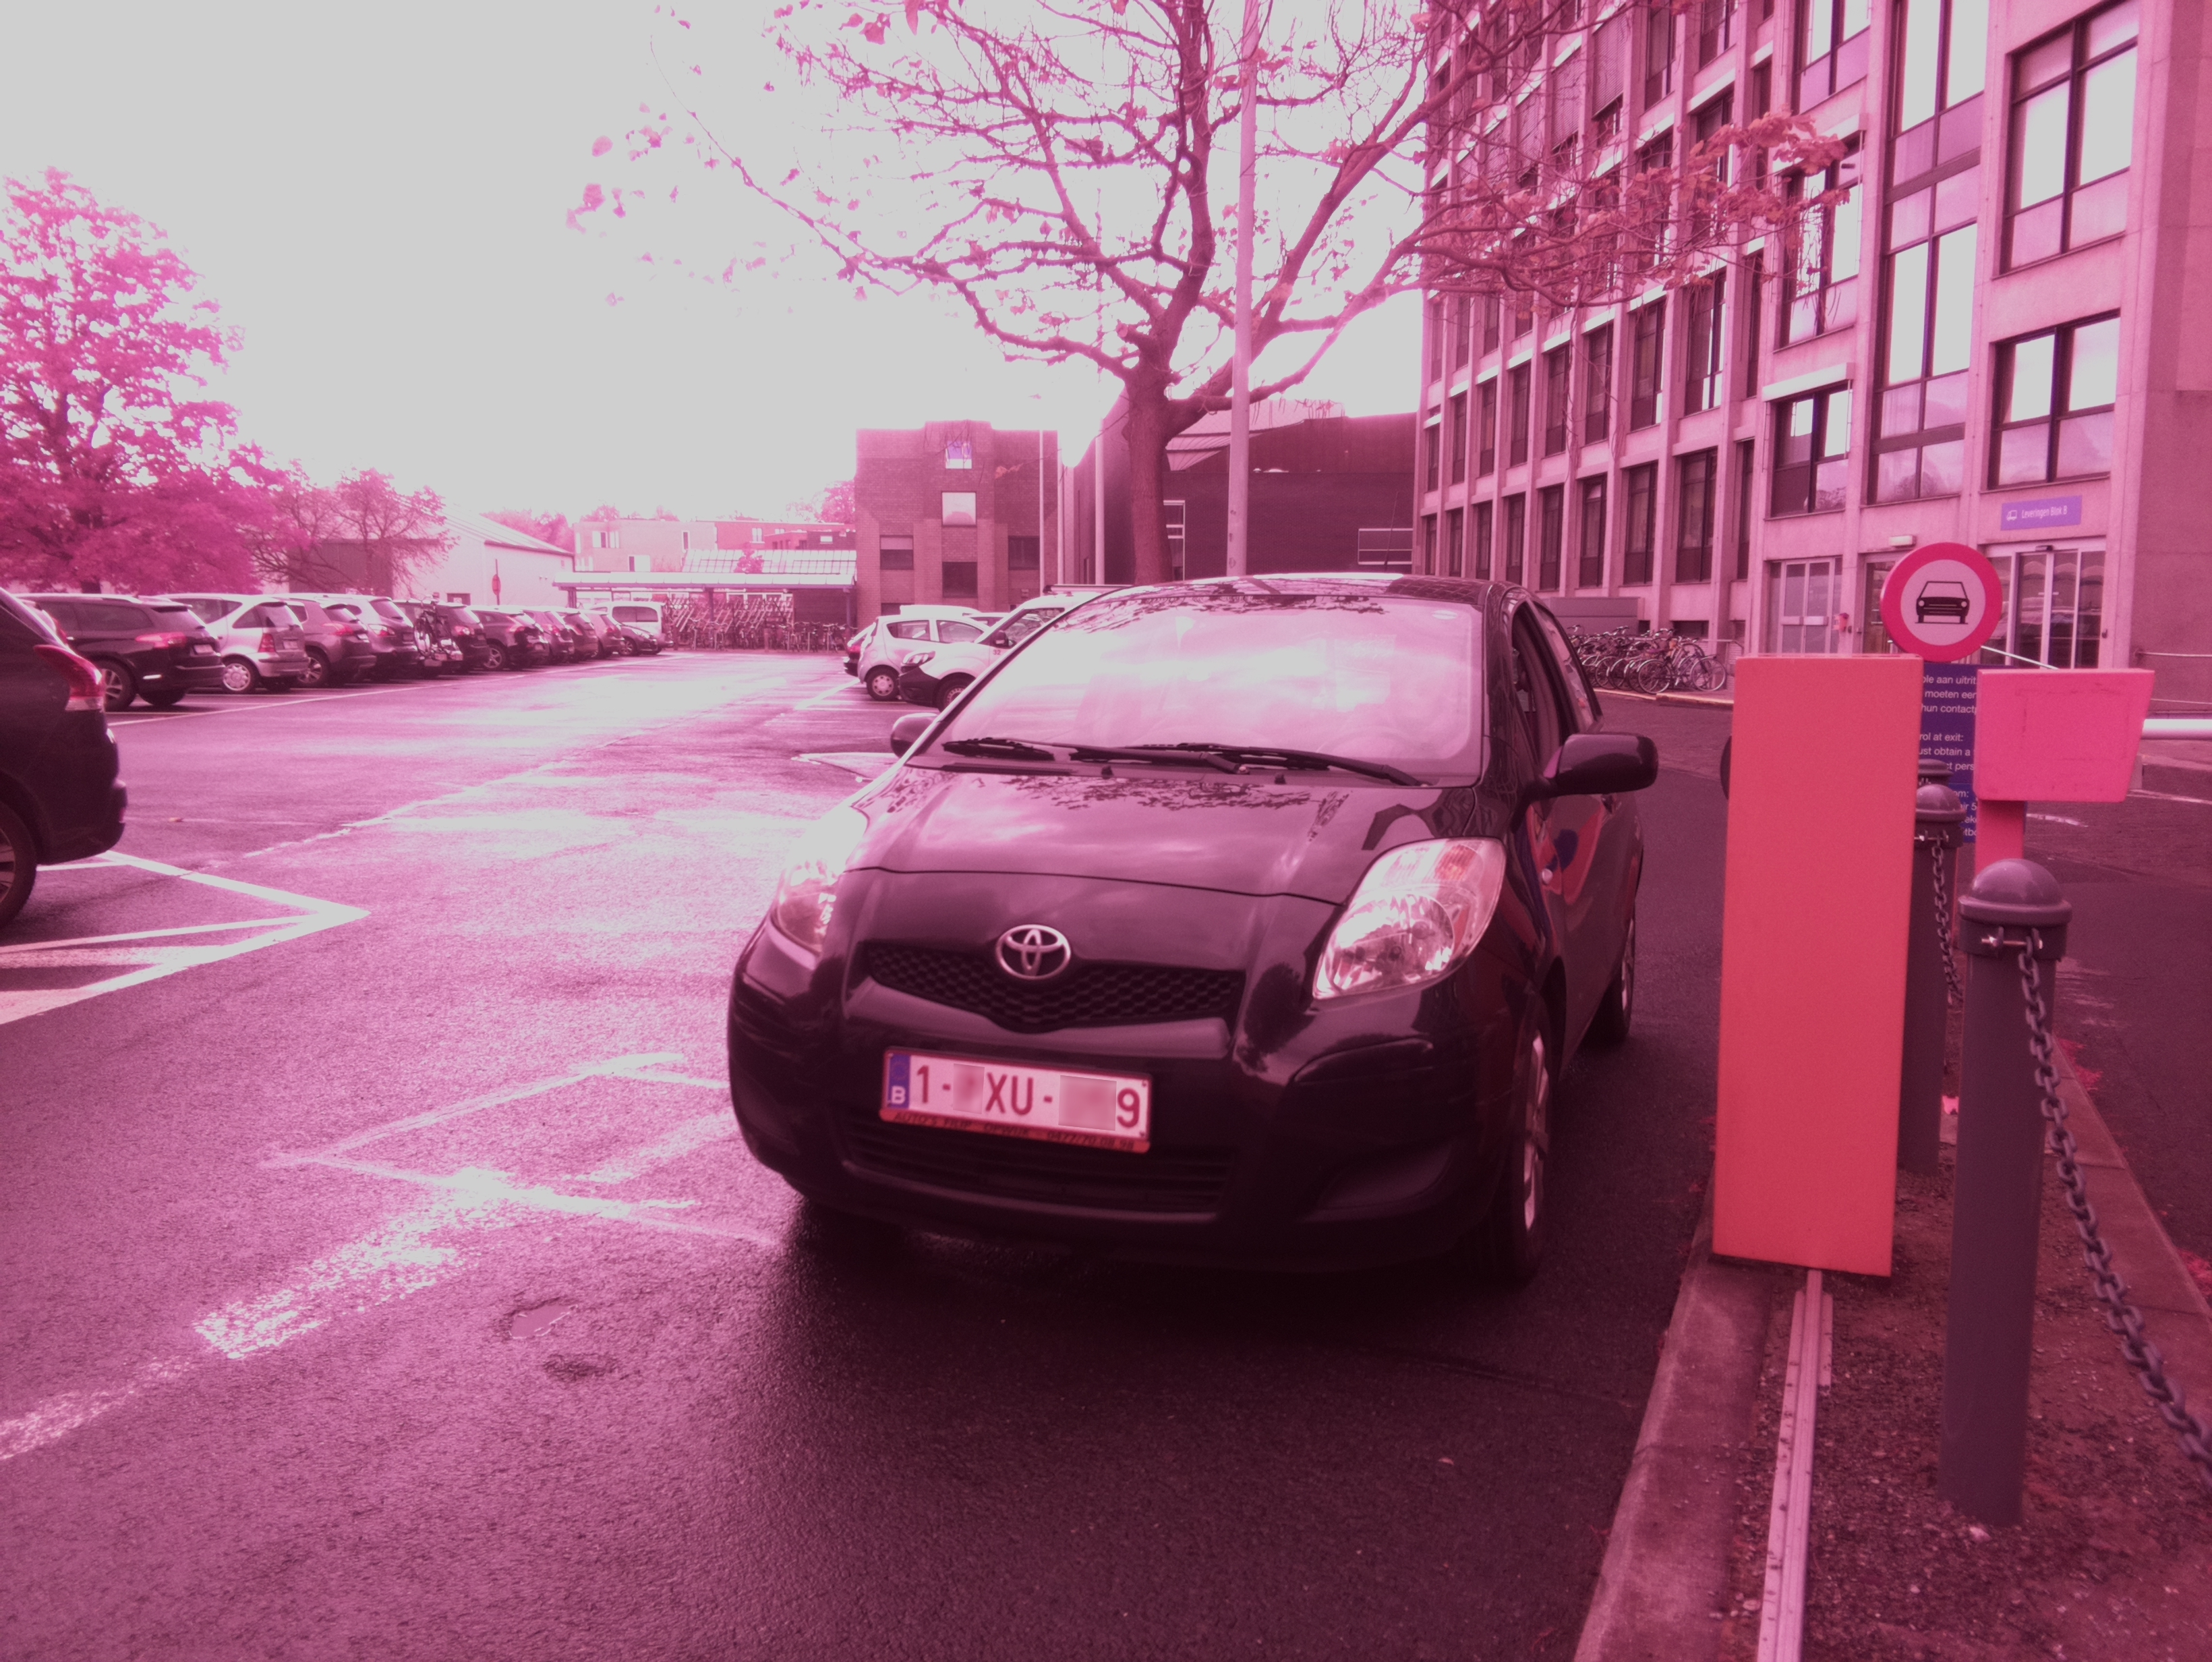
\includegraphics[width=0.7\linewidth]{img/kruisboog/kruisboog.jpg}
	\caption{Voorbeeld van een ANPR-foto aan de uitgang Kruisboogstraat. Enkele tekens van de nummerplaat zijn onleesbaar gemaakt uit privacy van de bestuurder.}
	\label{fig:Kruisboog}
\end{figure}

\subsubsection{Resultaten}

Met deze positie en camerahoek zijn de volgende resultaten bekomen:

\begin{table}[h!]
	\centering
	\begin{tabular}{l|l|l|l|l}
		\textbf{ANPR nauwkeurigheid: Kruisboogstraat} & Totaal & Incorrect & Correct & Ratio	\\ \hline
		Per individuele foto 	& 68 & 16 & 52	& 76.5\%\\
		Per auto				& 26 & 1 & 25		& 96.15\%\\
	\end{tabular}
	\caption{Resultaten van OpenALPR aan Campus Sterre - Uitgang Kruisboogstraat.}
	\label{ResultatenKruisboog}
\end{table}

De behaalde marge van 96.15\% is boven de gewenste nauwkeurigheid van 95\%. Waardoor besloten kan worden dat nummerplaatdetectie een haalbare technologie is aan de uitgang aan de Kruisboogstraat. Deze resultaten gelden enkel voor detectie overdag, zonder moeilijke weersomstandigheden.

\subsubsection{Fouten}
Op 1 auto na zijn alle auto's correct geïdentificeerd. De incorrecte afbeeldingen hebben geen merkwaardige verschillen van de andere afbeeldingen waardoor de juistheid lager zou liggen. We kunnen hieruit dus veronderstellen dat deze fout komt door de nauwkeurigheid van OpenALPR zelf. Mogelijks zou het verhogen van de resolutie van de camera een verbetering hebben op deze resultaten.

\begin{figure}[h!]
	\centering
	\includegraphics[width=0.8\linewidth]{img/kruisboog/kruisboog-incorrect.jpg}
	\caption{Een niet-geïdentificeerd voertuig aan de uitgang Kruisboogstraat. Enkele tekens van de nummerplaat zijn onleesbaar gemaakt uit privacy van de bestuurder.}
	\label{fig:kruisboog-incorrect}
\end{figure}

\subsection{Campus Coupure - Uitgang Coupure Links}
De uitgang aan de Coupure Links, afgebeeld in figuur \ref{fig:coupure-links}, had niet genoeg doorrijdende auto's om een degelijke steekproef te nemen, of een correcte cameraconfiguratie te vinden. Op een tijdsduur van 2u waren er in totaal 4 auto's gepasseerd. Het was niet mogelijk om de tijd te voorzien om genoeg foto's te verzamelen of om een opstelling te maken die achtergelaten kon worden. Hierdoor is deze uitgang niet verwerkt in dit onderzoek.

\begin{figure}[h!]
	\centering
	\includegraphics[width=0.8\linewidth]{img/coupure-links/coupure-links.jpg}
	\caption{Foto van de uitgang Coupure Links.}
	\label{fig:coupure-links}
\end{figure}

\section{Algemene resultaten}
%In het donker is de interferentie van de koplampen niet te groot, maar de algemene donkerheid van de omgeving zorgt ervoor dat de raspberry pi zijn shutter te lang openhoudt en dat de afbeeldingen enorm donker blijken. Het is dus vereist om extra infraroodbelichting bij te plaatsen.
%\begin{figure}[h!]
%	\centering
%	\includegraphics[width=0.5\linewidth]{img/nacht-coupure.jpg}
%	\caption{Onnauwkeurige foto's door een tekort aan licht.}
%	\label{SterreDonker}
%\end{figure}

\begin{table}[h!]
	\centering
	\begin{tabular}{l|l|l|l|l}
		\textbf{Resultaten per individuele foto}	& \textbf{Totaal}	& \textbf{Incorrect} & \textbf{Correct} & \textbf{Ratio} \\ \hline
		Campus Coupure - Uitgang Kruisboogstraat  & 68 & 16 & 52 & 76.5\% \\
		Campus Sterre - Uitgang Galglaan 		  & 62& 13 & 49 & 79.0\%\\
		Campus Sterre - Uitgang De Pintelaan	  & 64& 19 & 45 & 70.3\%\\ \hline
		Totaal 									  & 194& 48 & 146 & 75.3\%
	\end{tabular}
	\caption{Resultaten van nummerplaatdetectie per foto.}
	\label{tab:perpic}
\end{table}

\begin{table}[h!]
	\centering
	\begin{tabular}{l|l|l|l|l}
		\textbf{Resultaten per auto} & \textbf{Incorrect}	& \textbf{Correct} & \textbf{Aantal auto's} & \textbf{Ratio} \\ \hline
		Campus Coupure - Uitgang Kruisboogstraat& 1 & 25  & 26 & 96.15\% \\
		Campus Sterre - Uitgang Galglaan		& 1 & 22  & 23 & 95.7\%\\
		Campus Sterre - Uitgang De Pintelaan	& 2 & 24  & 26 & 92.0\%\\ \hline
		Totaal 									& 4 & 71 & 75 & 94.7\%
	\end{tabular}
	\caption{Resultaten van nummerplaatdetectie per auto.}
	\label{tab:percar}
\end{table}

Er werd in dit onderzoek vertrokken met de hypothese dat in een steekproef met nummerplaatdetectie een nauwkeurigheid boven de 95\% behaald kon worden. Dit resultaat was dan ook bevestigd bij twee van de drie beschreven uitgangen in tabel \ref{tab:percar}.

Een goedkope implementatie voor nummerplaatdetectie is dan ook in zekere mate mogelijk. Op twee van de drie geteste uitgangen is het mogelijk om de camera's op de metalen constructie naast de hefbomen te plaatsen en degelijke resultaten te behalen. Enkel op de uitgang aan de De Pintelaan is er noodzaak aan een uitgebreidere implementatie om de camera te kunnen monteren.

Aan de De Pintelaan voldeed de positie op de metalen constructie niet om degelijke resultaten te behalen en was een verhogen en verplaatsing noodzakelijk. Om nummerplaatdetectie aan deze uitgang te voorzien zou er dus een extra investering gemaakt moeten worden in het opzetten van een verhoging voor de camera en het leggen van kabels naar deze positie.

In het algemeen zijn de resultaten van dit onderzoek veelbelovend, maar kan er niet aangenomen worden dat deze gelden voor alle voertuigen op deze locaties. Toch stellen deze zeker de weg open naar breder onderzoek.

%\section{Uitbreidingen}
%Locatie van de sensor kan mss in het midden van balk \autocite{buhus2016automatic}.

%%=============================================================================
%% Conclusie
%%=============================================================================

\chapter{Conclusie}
\label{ch:conclusie}

% TODO: Trek een duidelijke conclusie, in de vorm van een antwoord op de
% onderzoeksvra(a)g(en). Wat was jouw bijdrage aan het onderzoeksdomein en
% hoe biedt dit meerwaarde aan het vakgebied/doelgroep? 
% Reflecteer kritisch over het resultaat. In Engelse teksten wordt deze sectie
% ``Discussion'' genoemd. Had je deze uitkomst verwacht? Zijn er zaken die nog
% niet duidelijk zijn?
% Heeft het onderzoek geleid tot nieuwe vragen die uitnodigen tot verder 
%onderzoek?

Het doel van dit onderzoek was het nagaan of nummerplaatdetectie een haalbare technologie was aan de UGent Campus Sterre en Campus Coupure. Dit met behulp van een Raspberry Pi met PiCam en de open-source implementatie van OpenALPR die een goedkope oplossing zouden kunnen bieden. Om deze vraag te beantwoorden werd onderzocht of een dergelijke implementatie mogelijk is met de intrede van de GDPR, en of deze wel degelijk goede resultaten kan opleveren op de uitgangen van de campussen zelf.

Om de eerste vraag te beantwoorden werd een literatuurstudie uitgevoerd over de GDPR zelf, dit hield in hoe deze werkt en hoe deze een ANPR-systeem beïnvloedt. Uit de studie bleek dat de wetgeving een zeer grote invloed heeft op een ANPR-detectie implementatie. Foto's en andere persoonsgegevens zijn verplicht zo min mogelijk verwerkt te worden en dit enkel indien dit gerechtvaardigd is. Verder moet het mogelijk zijn voor een betrokkene om deze op te vragen, te corrigeren of te verwijderen.

Een implementatie van een ANPR-systeem is wellicht haalbaar. De wettelijke gronden staat de verwerking van de foto's toe op de grond van het gerechtvaardigd belang zolang deze een duidelijke doelbinding hebben en niet voor andere zaken gebruikt worden. Functionaliteiten zoals het aanpassen van persoonsgegevens of het beveiligen van de gegevens zouden normaal gezien een hoge implementatiekost hebben om hier een systeem rond te bouwen. Maar door persoonsgegevens tot een absoluut minimum te houden en de betrokkene niet meer identificeerbaar te maken is deze functionaliteit niet vereist en dekt men implementatiekosten. Dit maakt het mogelijk om een implementatie goedkoop te maken en aldus haalbaar.

uit het andere literatuuronderzoek naar maatregelingen rond ANPR kwam  naar voor dat nummerplaatdetectie afhankelijk is van een zeer groot aantal factoren, waarvan camerainstellingen .

De technische implementatie haalde een verwachte nauwkeurigheid van gemiddeld 94.7\%, wat overeenkomt met het onderzoek van \textcite{figuerola2016automated}, waar men in optimale omstandigheden een nauwkeurigheid van 94.4\% behaalde. Het is niet mogelijk om aan te nemen dat dit resultaat overeenkomt met de volledige populatie, maar de goede resultaten stellen wel de weg open naar een breder onderzoek.

Voor de implementatie zelf is een relatief goedkope oplossing gevonden. Op twee van de uitgangen was het mogelijk om de camera gewoon op de metalen constructie van de hefboom te plaatsen, wat kosten omlaag brengt. Voor de uitgang aan de Campus Sterre Galglaan was dit helaas niet mogelijk door de vele inrijrichtingen en de interferentie van het zonlicht. Hierdoor is het essentieel om een verhoging of een paal te plaatsen om een degelijk resultaat te verkrijgen. Dit zal de kosten aan deze uitgang omhoog halen.

Ten laatste moet er benadrukt worden dat deze resultaten behaald zijn onder normale weersomstandigheden in zonlicht en lichte regen. Verder onderzoek is nodig om te bevestigen of een dergelijke implementatie succesvol is 's nachts of in hevige weersomstandigheden.

%%=============================================================================
%% Bijlagen
%%=============================================================================

\appendix
\renewcommand{\chaptername}{Appendix}

%%---------- Onderzoeksvoorstel -----------------------------------------------

\chapter{Onderzoeksvoorstel}

Het onderwerp van deze bachelorproef is gebaseerd op een onderzoeksvoorstel dat vooraf werd beoordeeld door de promotor. Dat voorstel is opgenomen in deze bijlage.

% Verwijzing naar het bestand met de inhoud van het onderzoeksvoorstel
%---------- Inleiding ---------------------------------------------------------

\section{Introductie} % The \section*{} command stops section numbering
\label{sec:introductie}

Parkings zijn van groot belang in het dagelijks leven. Iedere dag rijden talloze wagens naar hun plaats om daar na een achttal uren weer opgepikt te worden. Ieder van deze wagens moet zich dan ook telkens identificeren om deze te betreden of te verlaten. Dit doen ze met behulp van tickets, badges of andere toegangssystemen. Ieder systeem heeft zijn eigen voor- en nadelen.

Dit onderzoek wordt uitgevoerd met oog op de parking van UGent, waar men kampt met enkele problemen met de toegang van de parking aan de Campus Sterre en Campus Coupure. Momenteel worden er op deze parkings tokens en badges gebruikt om de parking te verlaten, welke enkele negatieve punten met zich meebrengen. Zo worden de tokens snel kwijtgeraakt en zijn deze duur om bij te maken. Deze tokens zijn ook universeel en kunnen gebruikt worden bij andere diensten die soortgelijke tokens gebruiken. Verder moeten deze slikkers regelmatig geleegd worden, wat dan weer een personeelskost met zich meebrengt. Men heeft al enkele oplossingen bekeken om dit systeem te vervangen en een grote favoriet is het gebruik van nummerplaatdetectie waarbij met een centraal systeem specifieke wagens toegang kunnen krijgen.
\\
Vele manieren van toegangscontrole zijn allicht mogelijk en niets is perfect. In dit onderzoek wordt gekeken naar welke toegangstechnieken haalbaar zijn en welke voordelen deze leveren. Ook zal met oog op de voorkeur van UGent dieper ingegaan worden op nummerplaatdetectie. Hierbij zal er gekeken worden hoe dit opgeleverd kan worden waarbij de General Data Protection Regulation (GDPR) nageleefd wordt en of dit haalbaar is om uit te voeren op lichte hardware zoals een Raspberry PI.

Zo bekomen we volgende onderzoeksvragen:
\begin{itemize}
	\item Welke toegangstechnieken brengen het meest profijt voor de parking van UGent?
	\item Is nummerplaatdetectie een haalbare techniek omtrent privacy en GDPR?
	\item Kan men nummerplaatdetectie uitvoeren op een Raspberry PI?
\end{itemize}

%---------- Stand van zaken ---------------------------------------------------

\section{State-of-the-art}
\label{sec:state-of-the-art}

% UGent hedendaags met tokens
Vandaag de dag kampt UGent met verscheidene problemen met hun huidige toegangssysteem. Hierbij kunnen gebruikers de parking vrij binnenrijden, maar om deze te verlaten moeten ze een token verschaffen aan de campus zelf. Deze token moet vervolgens ingeworpen worden in de tokenslikker aan de uitgang, waarna de gebruiker de parking kan verlaten. Deze tokens hebben weliswaar enkele nadelen. Zo worden deze snel kwijtgeraakt en moeten deze bijgemaakt worden, wat een redelijke kost is en niet milieubewust is. Ook zijn deze tokens universeel en kunnen in eender welke tokenslikker ingevoerd worden.
% Uitgang Campus Coupure met tickets
\subsection{Papieren tickets}
Door de problemen die bij het gebruik van tokens te kijk komen heeft men op Campus Sterre intussen één uitgang waar gebruikt gemaakt wordt van papieren tickets. Dit was bedoeld als alternatief voor de tokens, maar aangezien deze papieren tickets gelijkaardige problemen met zich meebrengen zou dit geen gewenste oplossing brengen.
% RFID scanners op UGent
\subsection{RFID}
Verder heeft iedere uitgang ook een RFID-scanner die gebruikt wordt om toegang te verlenen aan personeel. RFID kan m.b.v. een centraal systeem personeelskosten verminderen \autocite{pala2007smart}, maar op een campus waar men soms bezoekers voor maar één dag heeft is het niet wenselijk om hiervoor badges te bedelen.
% Mogelijkheid van nummerplaatdetectie
\subsection{Nummerplaatdetectie}
Een andere, nog niet geïmplementeerde techniek is nummerplaatdetectie. Deze techniek veroorzaakt geen directe milieubelasting aangezien er geen tickets of badges worden gebruikt, maar waar deze techniek wel onder lijdt is de zichtbaarheid van de nummerplaten in slechte weersomstandigheden \autocite{azam2016automatic}. Hierbij moet dus onderzocht worden in welke mate dit haalbaar is in deze case.
\\
Dit onderzoek zal nagaan welke toegangstechnieken het voordeligst zijn en welke het beste is in de case van UGent. Dit gebeurt a.d.h.v. een vergelijkende studie op vlak van benodigde werkuren, milieubelastbaarheid, transparantie voor opvolging en toegangscontrole. Verder zal er uitgebreid gekeken worden hoe nummerplaatdetectie gebruikt kan worden zodat deze niet in strijd zijn met wetgevingen zoals de privacywetgeving en de GDPR. Ten slotte zal er gekeken worden of dit uitgevoerd kan worden op een kleine microcontroller zoals de Raspberry pi 3 B+ en of deze kwalitatieve resultaten biedt.

% Voor literatuurverwijzingen zijn er twee belangrijke commando's:
% \autocite{KEY} => (Auteur, jaartal) Gebruik dit als de naam van de auteur
%   geen onderdeel is van de zin.
% \textcite{KEY} => Auteur (jaartal)  Gebruik dit als de auteursnaam wel een
%   functie heeft in de zin (bv. ``Uit onderzoek door Doll & Hill (1954) bleek
%   ...'')

%---------- Methodologie ------------------------------------------------------
\section{Methodologie}
\label{sec:methodologie}

Vooraleer de onderzoeksvragen beantwoord worden is er nood aan inzicht in verschillende mogelijke toegangstechnieken voor parkings. Dit zal gedaan worden a.d.h.v. een literatuurstudie, waarbij dan ook de eerste onderzoeksvraag zal beantwoord worden. In deze literatuurstudie zullen de karakteristieken op vlak van milieuvriendelijkheid, gebruiksvriendelijkheid en kost vergeleken worden. Vervolgens zal hieruit de keuze gemaakt worden welke techniek het beste is voor een parking met meerdere toegangspunten.

Om de tweede onderzoeksvraag te kunnen beantwoorden zal nog een literatuurstudie uitgevoerd worden omtrent privacy en GDPR. Het doel hiervan is om richtlijnen te bekomen voor het gebruik van camera’s op een parking zonder wetgevingen te overtreden.

Voor de laatste onderzoeksvraag zal onderzocht worden of nummerplaatdetectie een haalbare technologie is om te gebruiken op een Raspberry Pi 3B+. Dit zal getest worden door foto’s te nemen van voertuigen aan de toegangspunten aan UGent, waarna er gekeken wordt of deze nummerplaten detecteerbaar zijn met de Raspberry Pi. En of dit in een realistische tijd uitgevoerd kan worden met een acceptabele foutratio.

%---------- Verwachte resultaten ----------------------------------------------
\section{Verwachte resultaten}
\label{sec:verwachte_resultaten}

Er wordt verwacht dat nummerplaatdetectie het meest profijtelijk zal zijn in het geval van de parking van de UGent door de lagere kosten. Aan de toegangspunten zouden enkel camera’s en microcontrollers geïnstalleerd moeten worden, wat met de huidige netwerkinfrastructuur geen probleem moet zijn. Het implementeren van andere technieken zoals tickets zou ook een verbetering zijn, maar is nadeliger voor het milieu en brengt meer personeelswerk met zich mee zoals het legen van de slikkers en het aanvullen van de tickets. Voor nummerplaatdetectie foutmarge wordt verwacht dat 5\% van de inlezingen foutief zijn. Deze marge wordt genomen uit het onderzoek van \textcite{figuerola2016automated} waar men in optimale omstandigheden 94.4\% nauwkeurigheid gehaald heeft met gelijkaardige technologieen.

%---------- Verwachte conclusies ----------------------------------------------
\section{Verwachte conclusies}
\label{sec:verwachte_conclusies}

Indien de testresultaten van de nummerplaatdetectie hoog genoeg zijn en deze duidelijke voordelen heeft tegenover andere technieken, mogen we concluderen dat dit een haalbare toegangstechniek is voor de parking bij de UGent.


%%---------- Andere bijlagen --------------------------------------------------
% Voeg hier eventuele andere bijlagen toe
\chapter{R Code voor analyse per foto}
\lstinputlisting[basicstyle=\small]{bijlagen/alpr-per-pic.R}
\chapter{R Code voor analyse per auto}
\lstinputlisting[basicstyle=\small]{bijlagen/alpr-per-car.R}

%%---------- Referentielijst --------------------------------------------------

\printbibliography[heading=bibintoc]

\end{document}
